\documentclass{beamer}
\sloppy
\usepackage[utf8]{inputenc}
\usepackage[T1]{fontenc}
\usepackage{subcaption}
\usepackage{amsmath}
\usepackage{mathtools} 
\usepackage{empheq}
\usepackage[most]{tcolorbox}
\usepackage{adjustbox}
\usepackage{hyperref}

%%%%%%%%%%%%%%%%%%%%%%%%%%%%%%%%
% Custom commands
%%%%%%%%%%%%%%%%%%%%%%%%%%%%%%%%
\newtcbox{\mymath}[1][]{%
    nobeforeafter, math upper, tcbox raise base,
    enhanced, colframe=blue!30!black,
    colback=blue!30, boxrule=1pt,
    #1}

\title{A Bayesian approach to assess the spread of COVID-19 using an extended SEIRD model with implicit quarantine mechanism}
\subtitle{Applications in Brazilian locations}
\date[eSMB 2020]{SMB 2020 Annual Meeting}
\author[Diego T. Volpatto]{
	\textbf{Diego T. Volpatto}\inst{1}, Anna Claudia M. Resende\inst{1}, \\
	Lucas dos Anjos\inst{1}, Jo\~ao Vitor O. Silva\inst{1}, Claudia M. Dias\inst{2}, \\
	Regina C. Almeida\inst{1}, Sandra M. C. Malta\inst{1}
}
% \author[Anna Claudia]{
% 	\textbf{Anna Claudia M. Resende}\inst{1}
% }

\institute[LNCC] % Your institution as it will appear on the bottom of every slide, may be shorthand to save space
{
\inst{1} Laboratório Nacional de Computação Científica (LNCC) \\ % Your institution for the title page
\inst{2} Universidade Federal Rural do Rio de Janeiro (UFRRJ)
}

\usetheme{lncc}

\begin{document}

\begin{frame}
\titlepage
\end{frame}

\begin{frame}
\frametitle{Agenda} % Table of contents slide, comment this block out to remove it
\tableofcontents % Throughout your presentation, if you choose to use \section{} and \subsection{} commands, these will automatically be printed on this slide as an overview of your presentation
\end{frame}

\section{COVID-19 in Brazil}

\subsection{What is happening?}

\begin{frame} 
\frametitle{COVID-19 in Brazil} 
\framesubtitle{What is happening?} 
\begin{block}{Brazil's non-pharmaceutical interventions (NPIs)}
	\begin{itemize}
		\item Moderate social distancing measures
		\item Weak quarantine policies
		\item Lack of vaccines/medicines
		\item Underreporting and undertesting
	\end{itemize}
\end{block}
\end{frame}

\subsection{The numbers (do you mean "human beings"?)}

\begin{frame} 
\frametitle{COVID-19 in Brazil} 
\framesubtitle{The numbers (do you mean "human beings"?)} 

\begin{center}
    Date: 19/08/2020
\end{center}

\begin{columns}
\begin{column}{0.5\textwidth}
    \begin{center}
    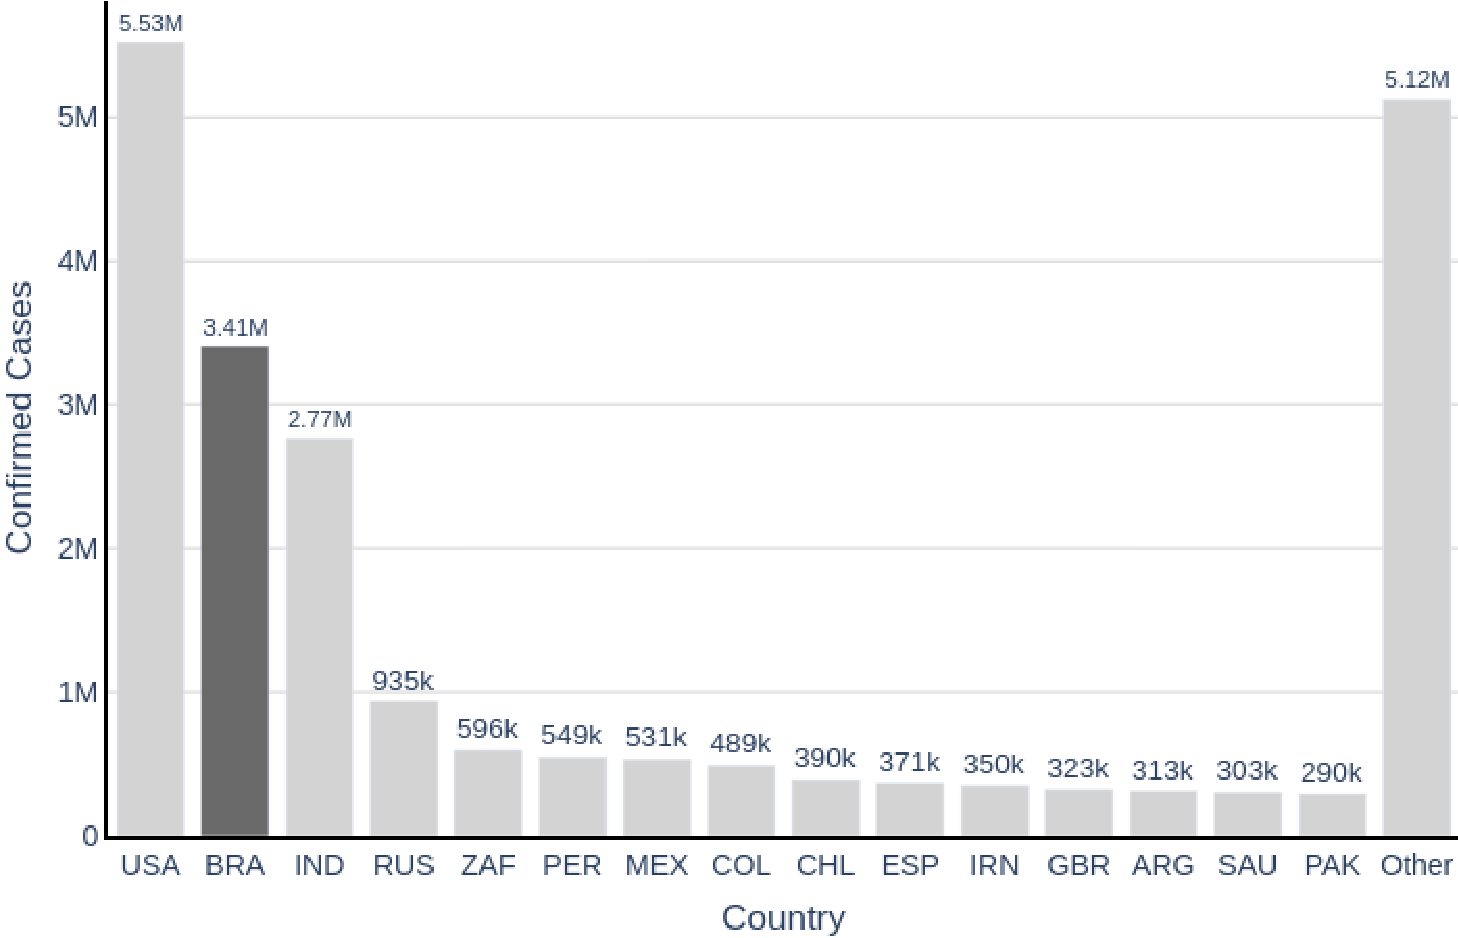
\includegraphics[width=1\textwidth]{figs/new_confirmed.pdf}
    \end{center}
\end{column}
\begin{column}{0.5\textwidth}  %%<--- here
    \begin{center}
    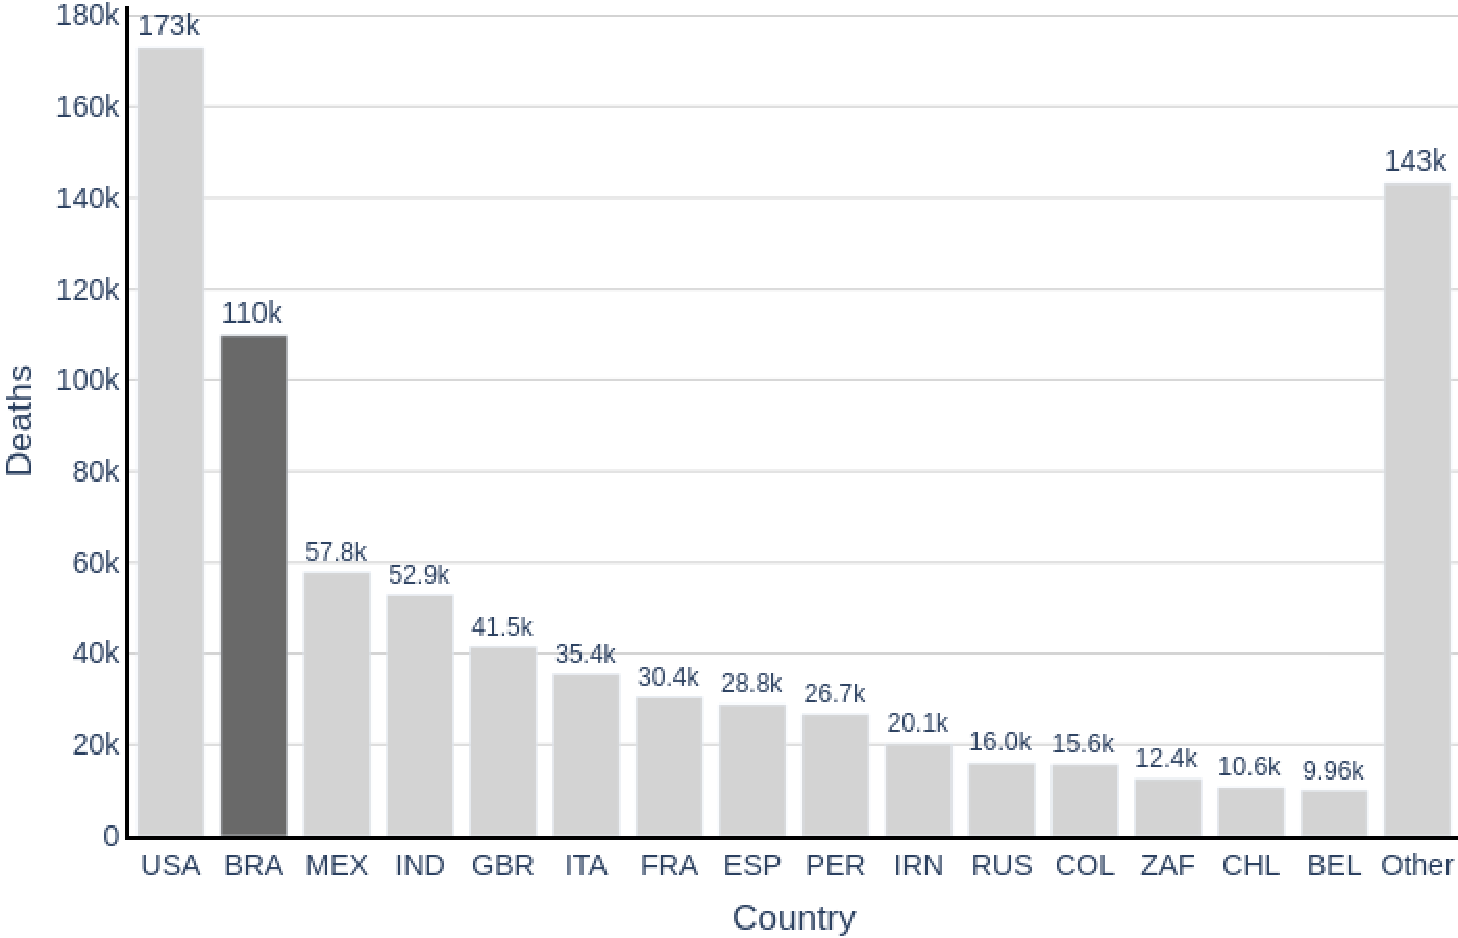
\includegraphics[width=1\textwidth]{figs/new_deaths.pdf}
    \end{center}
\end{column}
\end{columns}

\vspace{2em}

\begin{center}
    These numbers are in "human beings" unit!!!
\end{center}

\end{frame}

\subsection{What we could do as scientists?}

\begin{frame} 
\frametitle{COVID-19 in Brazil} 
\framesubtitle{What we could do as scientists?} 
\begin{itemize}
    \item The question that comes to mind: \textbf{What we could do as scientists?}
    \item Forecasting is really hard! What if it does not match with reality afterward?
    \item Understanding is the "key" to open the "door" of actions
    \item With understanding of a phenomenon, you can \textbf{advise}!
    \item Our general goal: to \textbf{advise} (not forecast!) based on \textbf{scientific evidence}
    \item Our specific goal: to advise about NPIs and, more specifically, about \textbf{quarantine policies}
\end{itemize}
\end{frame}

\section{An extended SEIRD model}

\subsection{What we want to understand?}

\begin{frame} 
\frametitle{An extended SEIRD model} 
\framesubtitle{What we want to understand?} 

\begin{itemize}
    \item Models are \textbf{simplifications/approximations} of reality
    \item \textit{"All models are wrong, but some are useful"} (attributed to G. Box)
    \item Modeling goals: understanding some \textbf{features of reality} (not all!)
    \item \textbf{This work} $\to$ To understand the effect of \textbf{quarantine} on COVID-19 spreading in \textbf{Brazil (country)} and \textbf{Rio de Janeiro state}
\end{itemize}

\end{frame}

\subsection{SEAIRPD-Q model in a glance}

\begin{frame} 
\frametitle{An extended SEIRD model} 
\framesubtitle{SEAIRPD-Q model} 

\begin{figure}
	\centering
	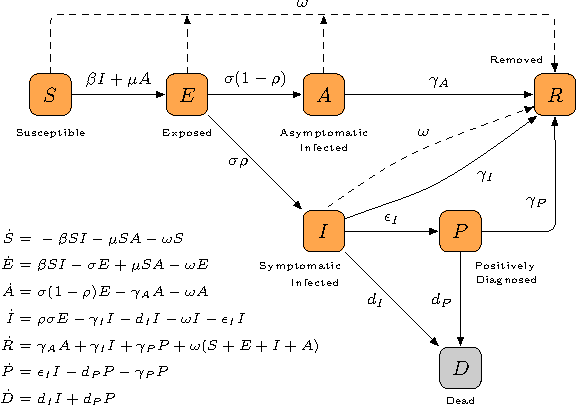
\includegraphics[width=1\textwidth]{./figs/final_schem_no_eta-crop.pdf}
\end{figure}

\end{frame}

\section{Sensitivity and Uncertainties}

\subsection{How we find the most influential parameters?}

\begin{frame}{\insertsubsection}
\frametitle{Sensitivity and Uncertainties} 
\framesubtitle{How we find the most influential parameters?} 
	\begin{block}{Sensitivity analysis goals}
		\begin{itemize}
			\item How changes in model factors affect QoIs?
			\item Assess model factors' importance
			\item Help to understand how the model response to perturbations
		\end{itemize}
	\end{block}
	\vspace{1em}
	
	\begin{minipage}[b]{0.49\textwidth}
		\begin{center} \textbf{Effective Reproduction number}
			\begin{empheq}[box={\mymath[colback=lncc-color!20, drop lifted shadow]}]{equation*}
			\text{QoI}_1(t) = \mathcal{R}(t)
			\end{empheq}
		\end{center}
	\end{minipage}\hfill
	\begin{minipage}[b]{0.49\textwidth}
		\begin{center} \textbf{Normalized squared sum}
			\begin{empheq}[box={\mymath[colback=lncc-color!20, drop lifted shadow]}]{equation*}
			\text{QoI}_2(t) = \sqrt{C(t)^2 + D(t)^2}
			\end{empheq}
		\end{center}		
	\end{minipage}
	
%	\vspace{.15in} \begin{center} \large \underline{\bf Hip\'oteses} \end{center}
	\vspace{0.2in}
	\begin{itemize}
		\item Enhanced \textbf{Elementary Effects method} (Campolongo et al., 2007) using \texttt{SALib}
		\item Factors' distributions: $\theta_i \sim \mathcal{U}(0.5\bar{\theta}_i, 1.5\bar{\theta}_i)$

	\end{itemize}
\end{frame}

\subsection{How uncertainties are taken into account?}

\begin{frame}
\frametitle{Sensitivity and Uncertainties} 
\framesubtitle{How uncertainties are taken into account?} 

\begin{itemize}
	\item Fitting parameters ($\boldsymbol{\theta}$): $\{\beta=\mu, d_I, d_P, \omega\}$ and $\{\sigma_C, \sigma_D\}$
	\item Noise on data: $\mathcal{N} (0,\sigma_C^2)$ e $\mathcal{N} (0, \sigma_D^2)$		
	\item Observed quantities $C$ and $D$:
\end{itemize}
	
\begin{center} 
    \textbf{Likelihood function}
\end{center}

\vspace{-2.5em}
\begin{empheq}[box={\mymath[colback=lncc-color!20, drop lifted shadow]}]{equation*}\small
	\pi_{\text{like}}(\boldsymbol{y}|\boldsymbol{\theta}) = \prod_{j\in \{C,D\} } 	{\dfrac{1}{\sigma_j\sqrt{2\pi}}}\exp\left( - \frac{1}{2} \sum_{i = 1}^n \left( \frac{y^{(j)}(t_i) - y_{\text{model}}^{(j)}(t_i)} {\sigma_j} \right)^2 \right)
\end{empheq}
	
% \vspace{1em}
\begin{itemize}
	\item Bayesian calibration: CATMIP (\textit{Cascading Adaptive Transitional Metropolis in Parallel}) from \texttt{PyMC3}
\end{itemize}
\end{frame}

\section{Results}

\subsection{Data source and Code}

\begin{frame}
\frametitle{Results} 
\framesubtitle{Data source and Code} 

\begin{itemize}
    \item Data for model calibration:
    \begin{itemize}
        \item \underline{\textbf{Brazil (Health Ministry)}}: \url{https://covid.saude.gov.br/}
        \item RJ state: \url{https://covid19br.wcota.me/}
        \item Data range: March-May (approximately 2 months)
    \end{itemize}
    \item Code:
    \begin{itemize}
        \item Open Source
        \item Code and Data available at: \url{https://doi.org/10.5281/zenodo.3865730}
    \end{itemize}
\end{itemize}

\end{frame}

\subsection{Which are the most important factors?}

\begin{frame}
\frametitle{Results} 
\framesubtitle{Which are the most important factors?} 
\begin{itemize}
    \item Sensitivity measures here: normalized mean of the absolute overall factor influence on QoI for different times
\end{itemize}
	
	\begin{figure}
		\centering
		\begin{subfigure}[t]{0.49\textwidth}
			\centering
			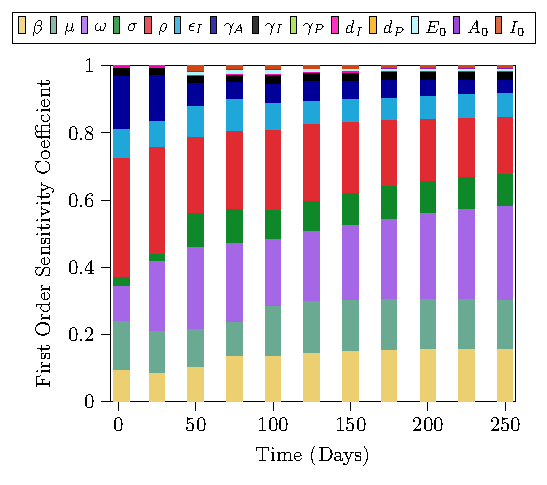
\includegraphics[width=\textwidth]{figs/EE_Brasil_Rt.pdf}
			\caption*{$\text{QoI}_1(t)$}
		\end{subfigure}
		\hfill
		\begin{subfigure}[t]{0.49\textwidth}
			\centering
			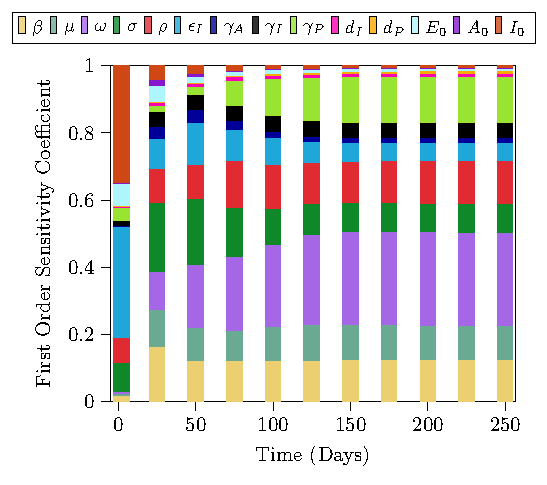
\includegraphics[width=\textwidth]{figs/EE_Brasil_CtDt.pdf}
			\caption*{$\text{QoI}_2(t)$}
		\end{subfigure}
	\end{figure}
\end{frame}

\subsection{Assessing quarantine scenarios}

\begin{frame}
\frametitle{Results} 
\framesubtitle{Assessing quarantine scenarios} 

	\begin{block}{Quarantine scenarios - what happens if...}

		\begin{enumerate}
			\item Relaxation of quarantine policy before infection peak:
			\begin{itemize}
			    \item Abrupt release
			    \item Progressive relaxation
			\end{itemize}
			\item Relaxation of quarantine policy after infection peak:
			\begin{itemize}
			    \item Abrupt release
			    \item Progressive relaxation
			\end{itemize}
		\end{enumerate}
	\end{block}
	
	\makebox[\textwidth][c]{
		\begin{minipage}[b]{0.57\textwidth}
			\begin{center} \textbf{Removal/quarantine rate}
				\begin{empheq}[box={\mymath[colback=lncc-color!20, drop lifted shadow]}]{equation*}
					\omega_r = \omega e^{-\lambda(t - t_d)}
				\end{empheq}
				{\small \textbf{Decay constant:} $\lambda = \ln2/t_{1/2}$;}\\
				{\small \textbf{Release day:} $t_d$;}
			\end{center}
		\end{minipage}
		\begin{minipage}[b]{0.35\textwidth}
			\begin{figure}
				\begin{tikzpicture}
					\node[circle, draw, label=above:{\small COVID-19}, inner sep=1.0cm, line width=0.4mm, fill tile image*={width=5.65cm}{figs/covid.jpg}] (A) {};
				\end{tikzpicture}
			\end{figure}
	\end{minipage}}

\end{frame}


\begin{frame}
\frametitle{Results} 
\framesubtitle{Assessing quarantine scenarios} 

	\begin{figure}
		\centering
		\caption*{Relaxation after infection peak (disease spreading under control)}
		\begin{subfigure}[t]{0.49\textwidth}
			\centering
            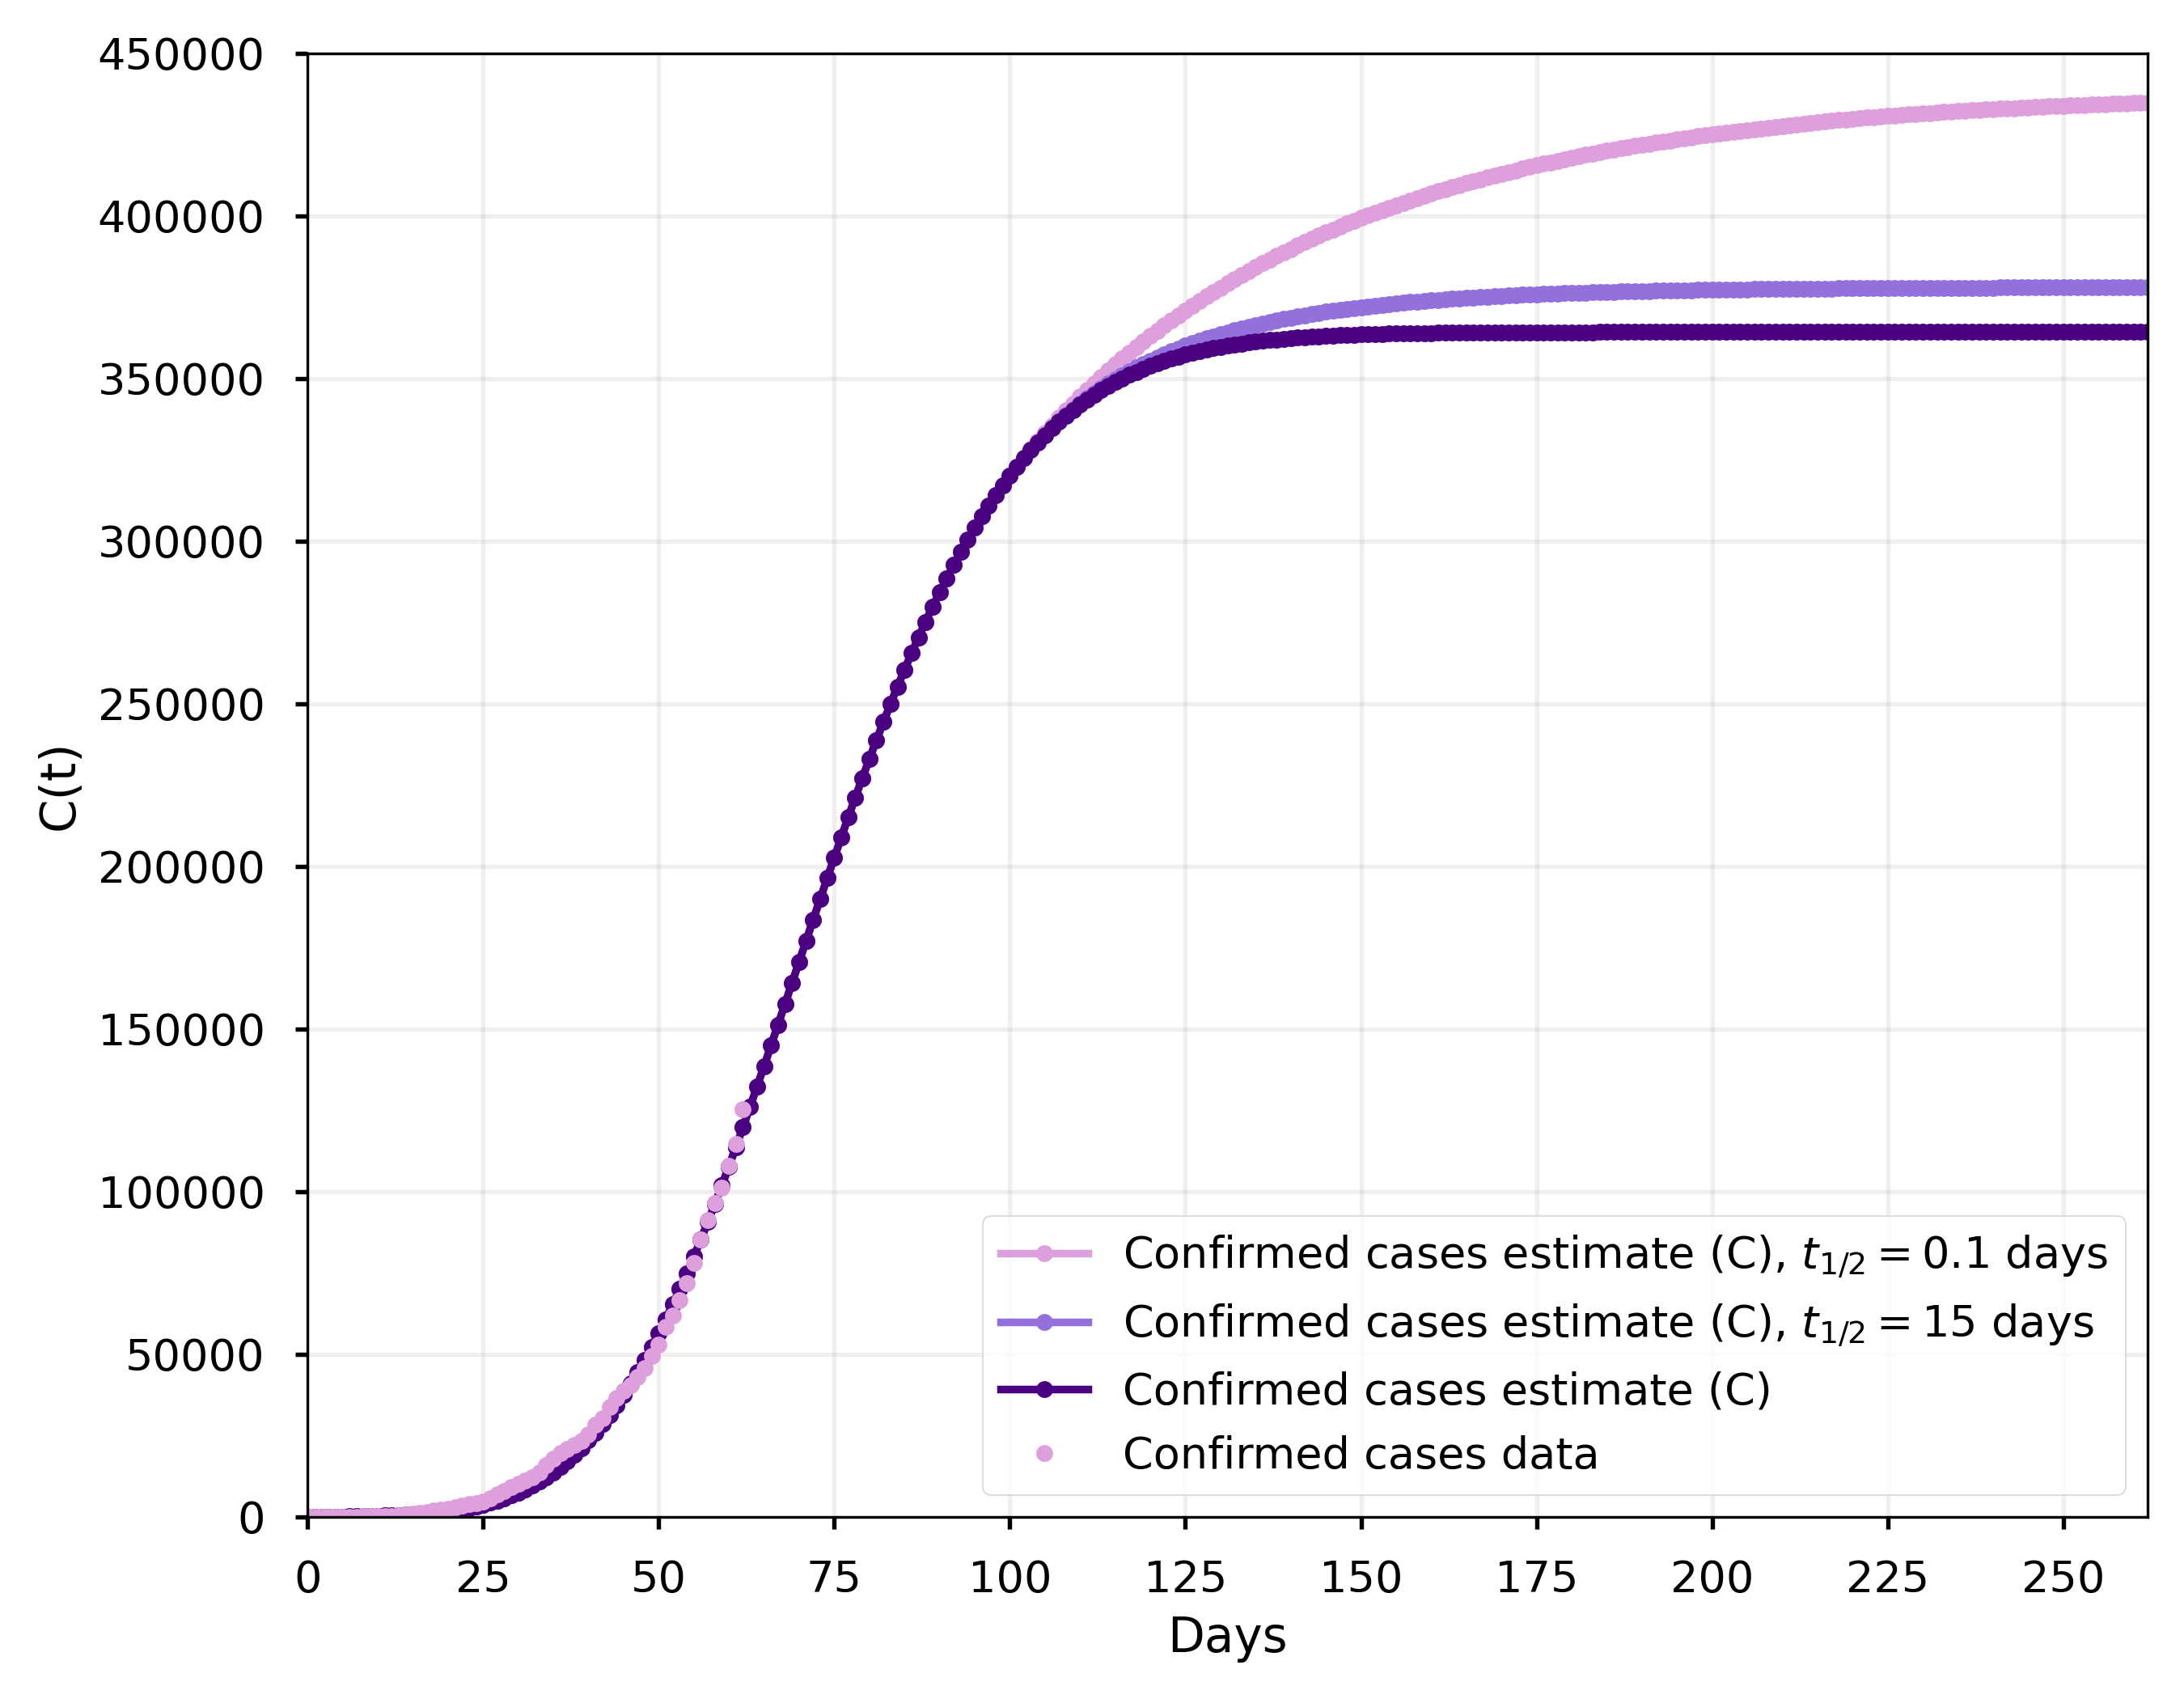
\includegraphics[width=\textwidth]{figs/model_prediction_mean_confirmed.png}
			\caption*{Confirmed cases}
		\end{subfigure}
		\hfill
		\begin{subfigure}[t]{0.49\textwidth}
			\centering
			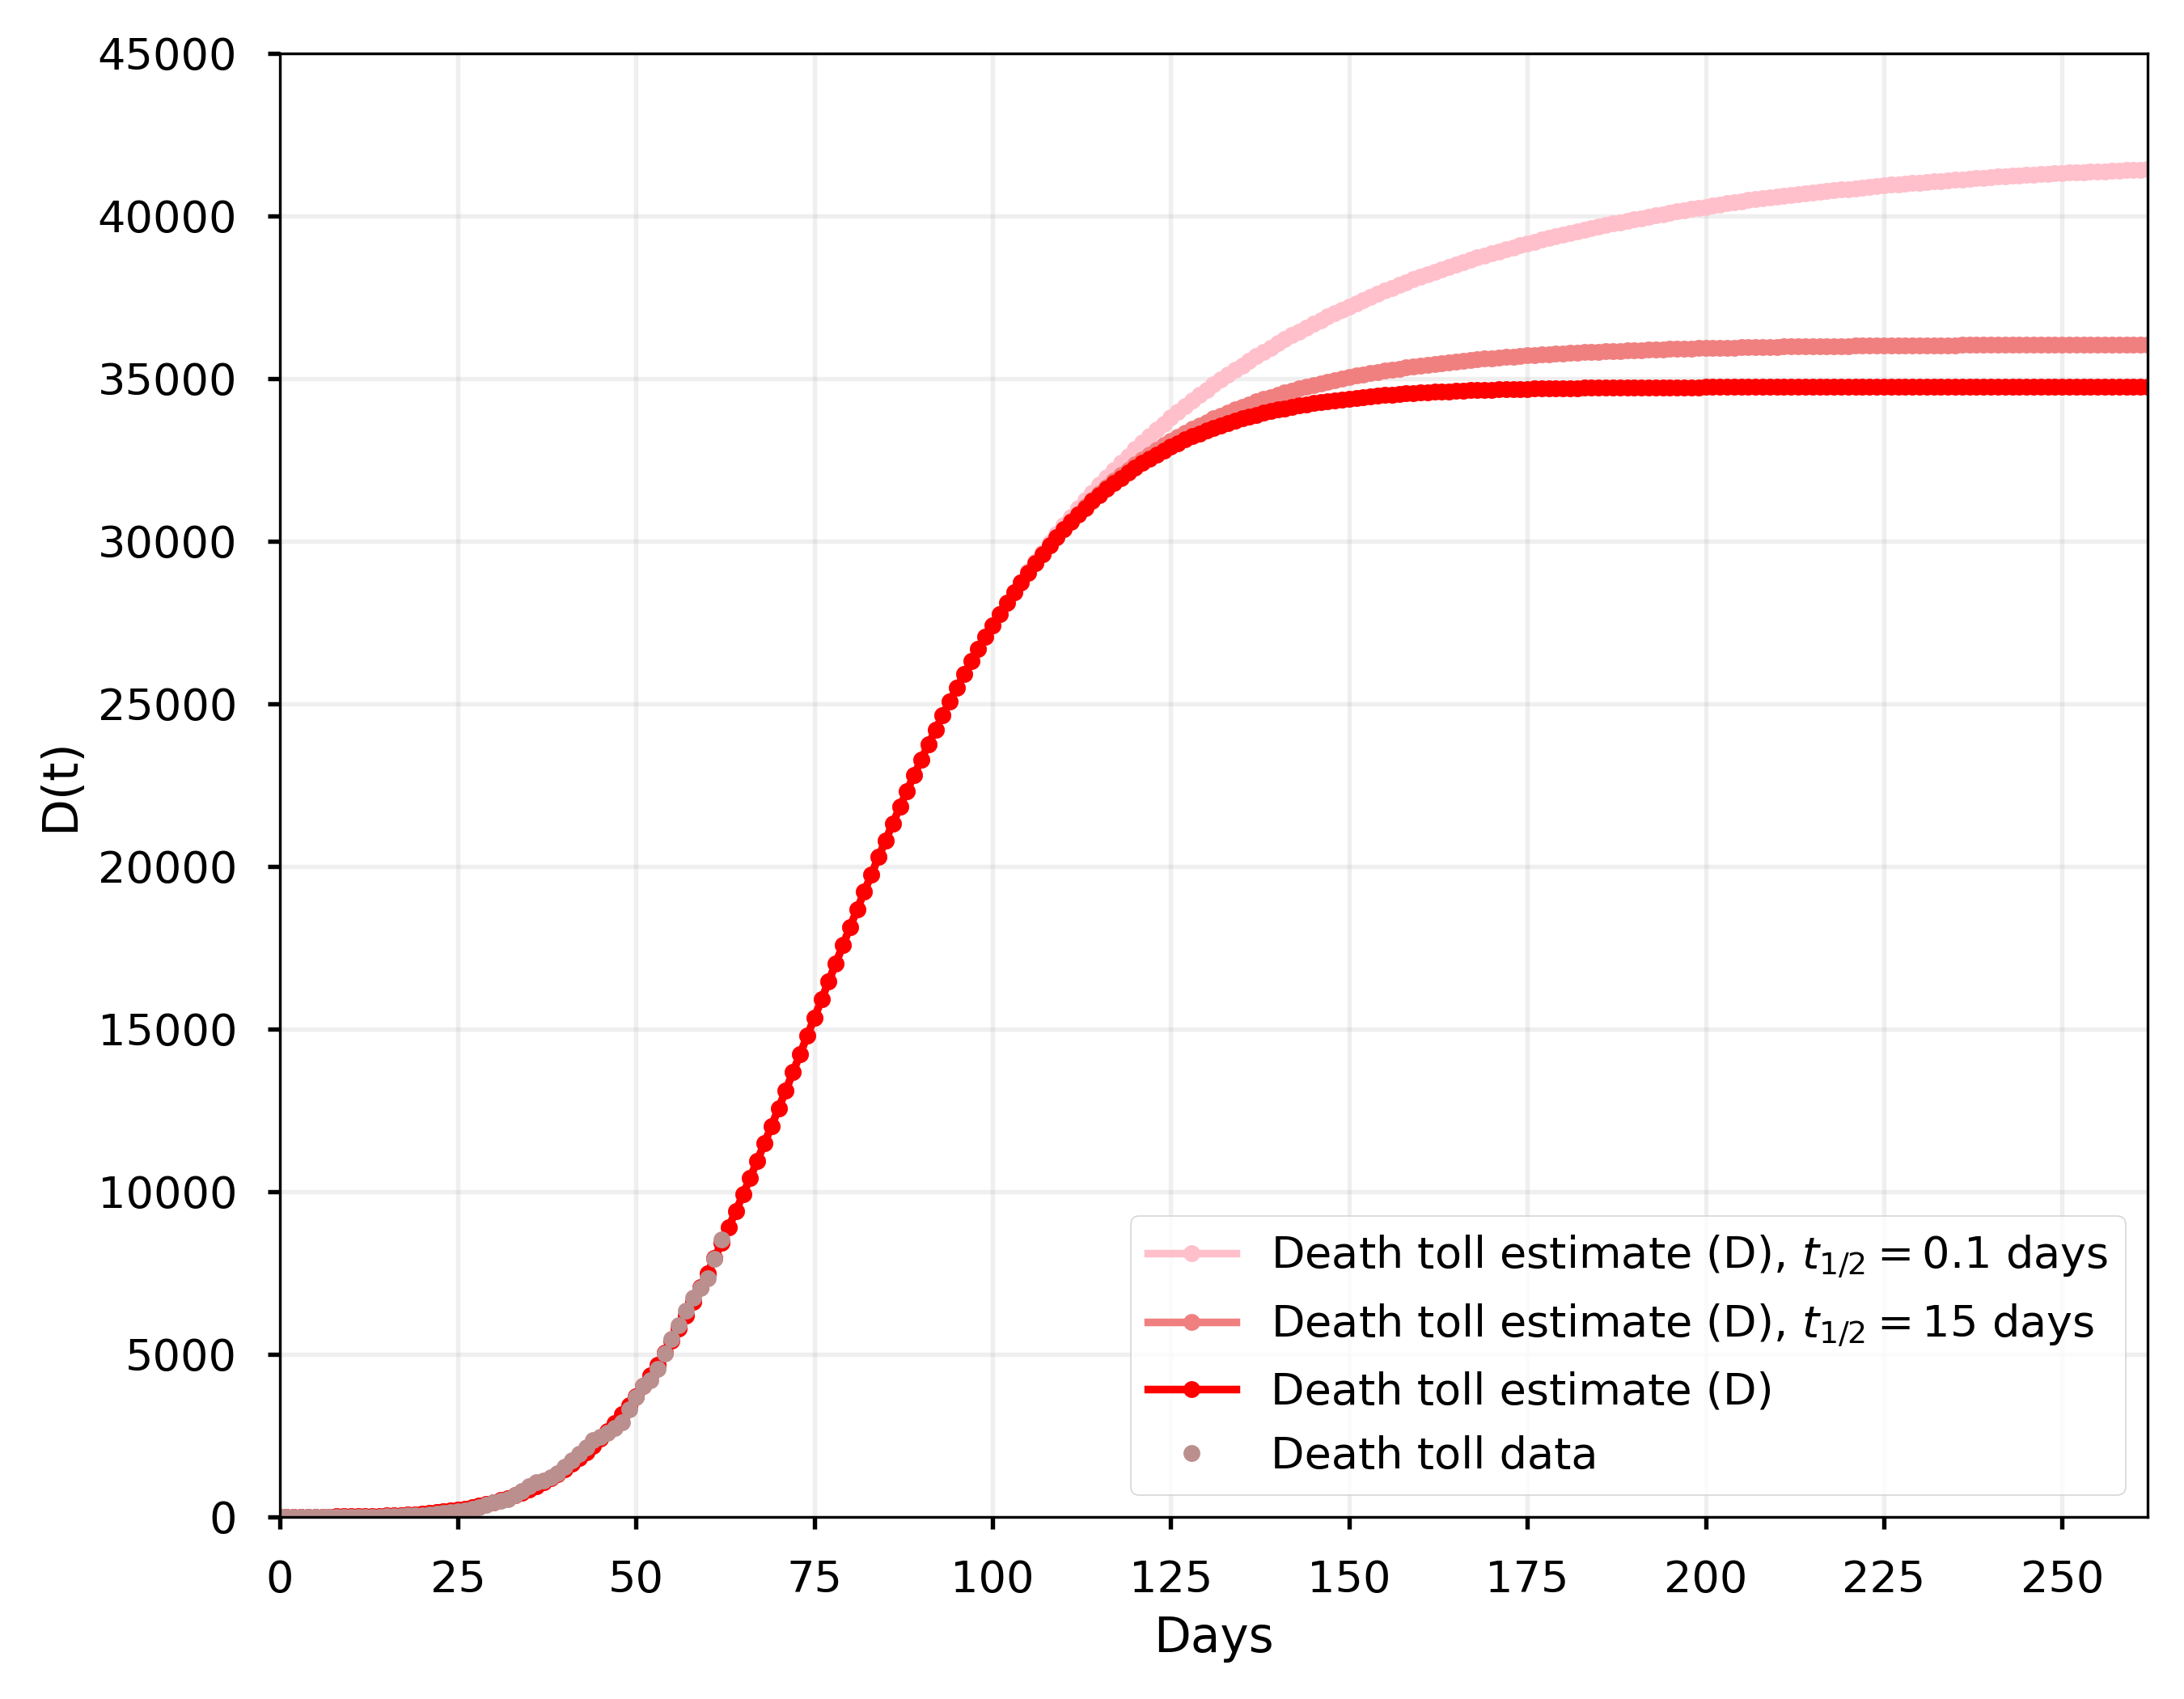
\includegraphics[width=\textwidth]{figs/model_prediction_mean_dead.png}
			\caption*{Death toll}
		\end{subfigure}
	\end{figure}

\end{frame}

\begin{frame}
\frametitle{Results} 
\framesubtitle{Assessing quarantine scenarios} 

	\begin{figure}
		\centering
		\caption*{When disease spreading ends...}
		\begin{subfigure}[t]{0.49\textwidth}
			\centering
			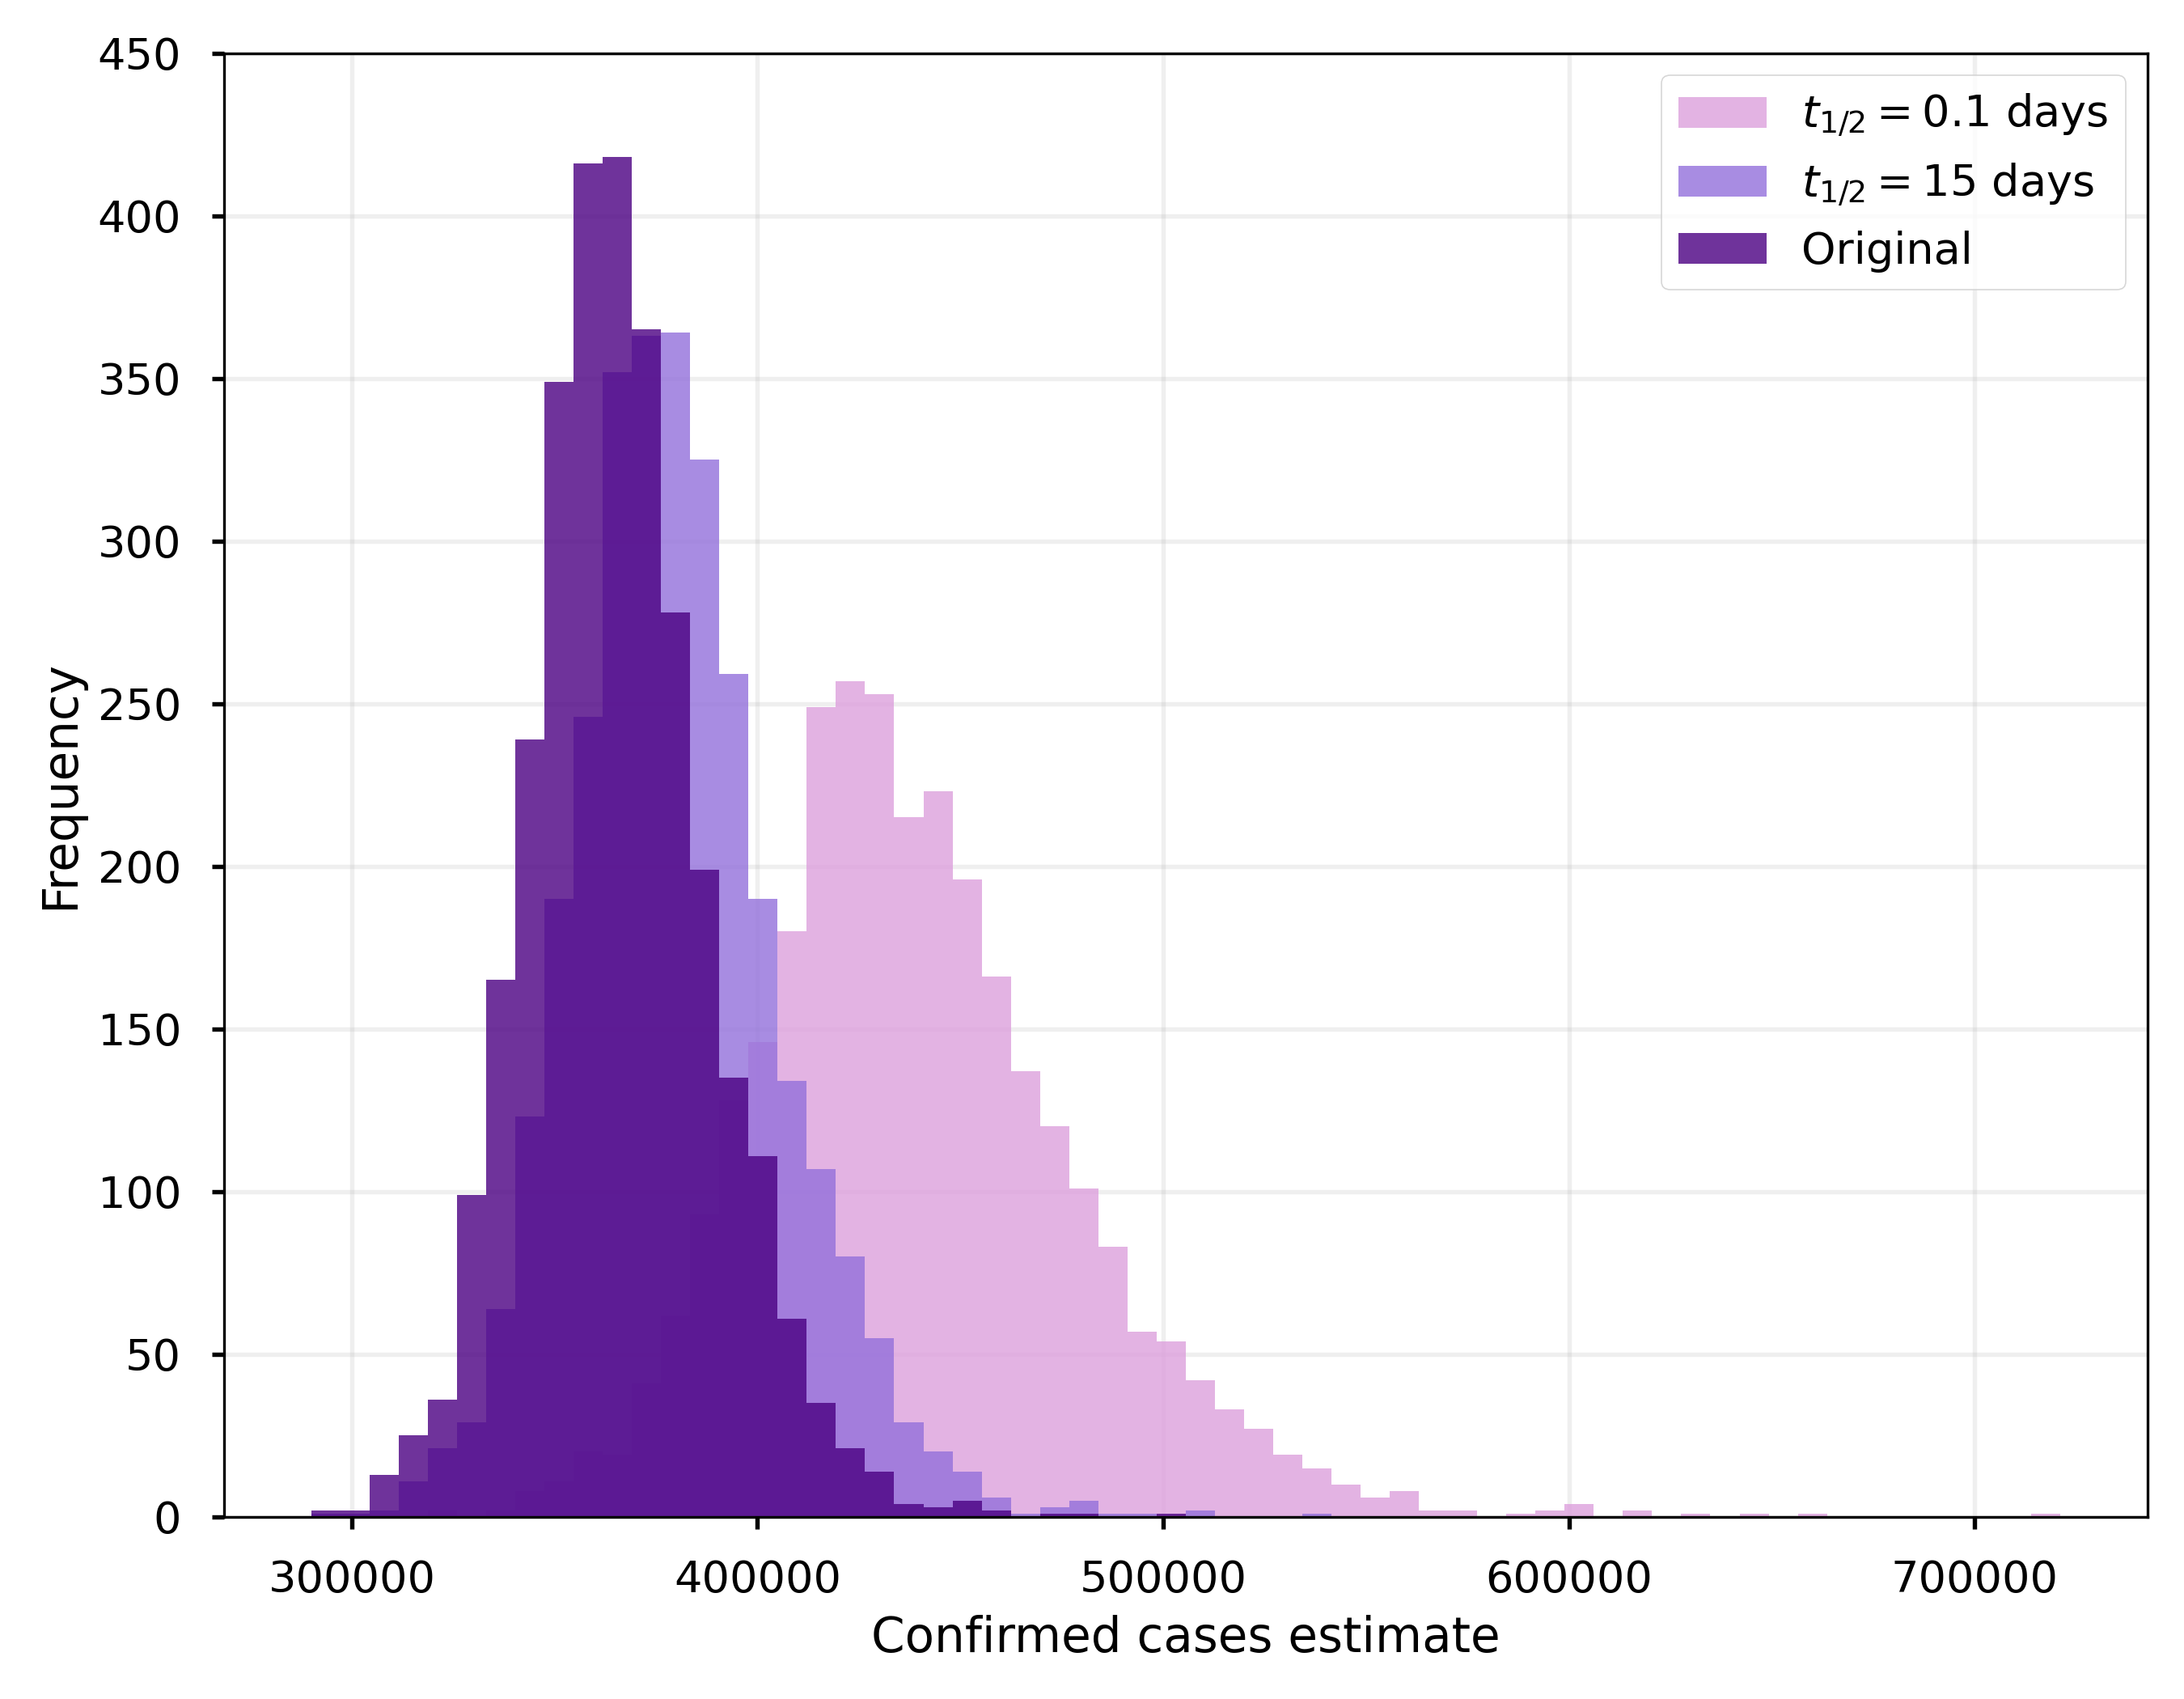
\includegraphics[width=\textwidth]{figs/model_prediction_confirmed.png}
			\caption*{Confirmed cases}
		\end{subfigure}
		\hfill
		\begin{subfigure}[t]{0.49\textwidth}
			\centering
			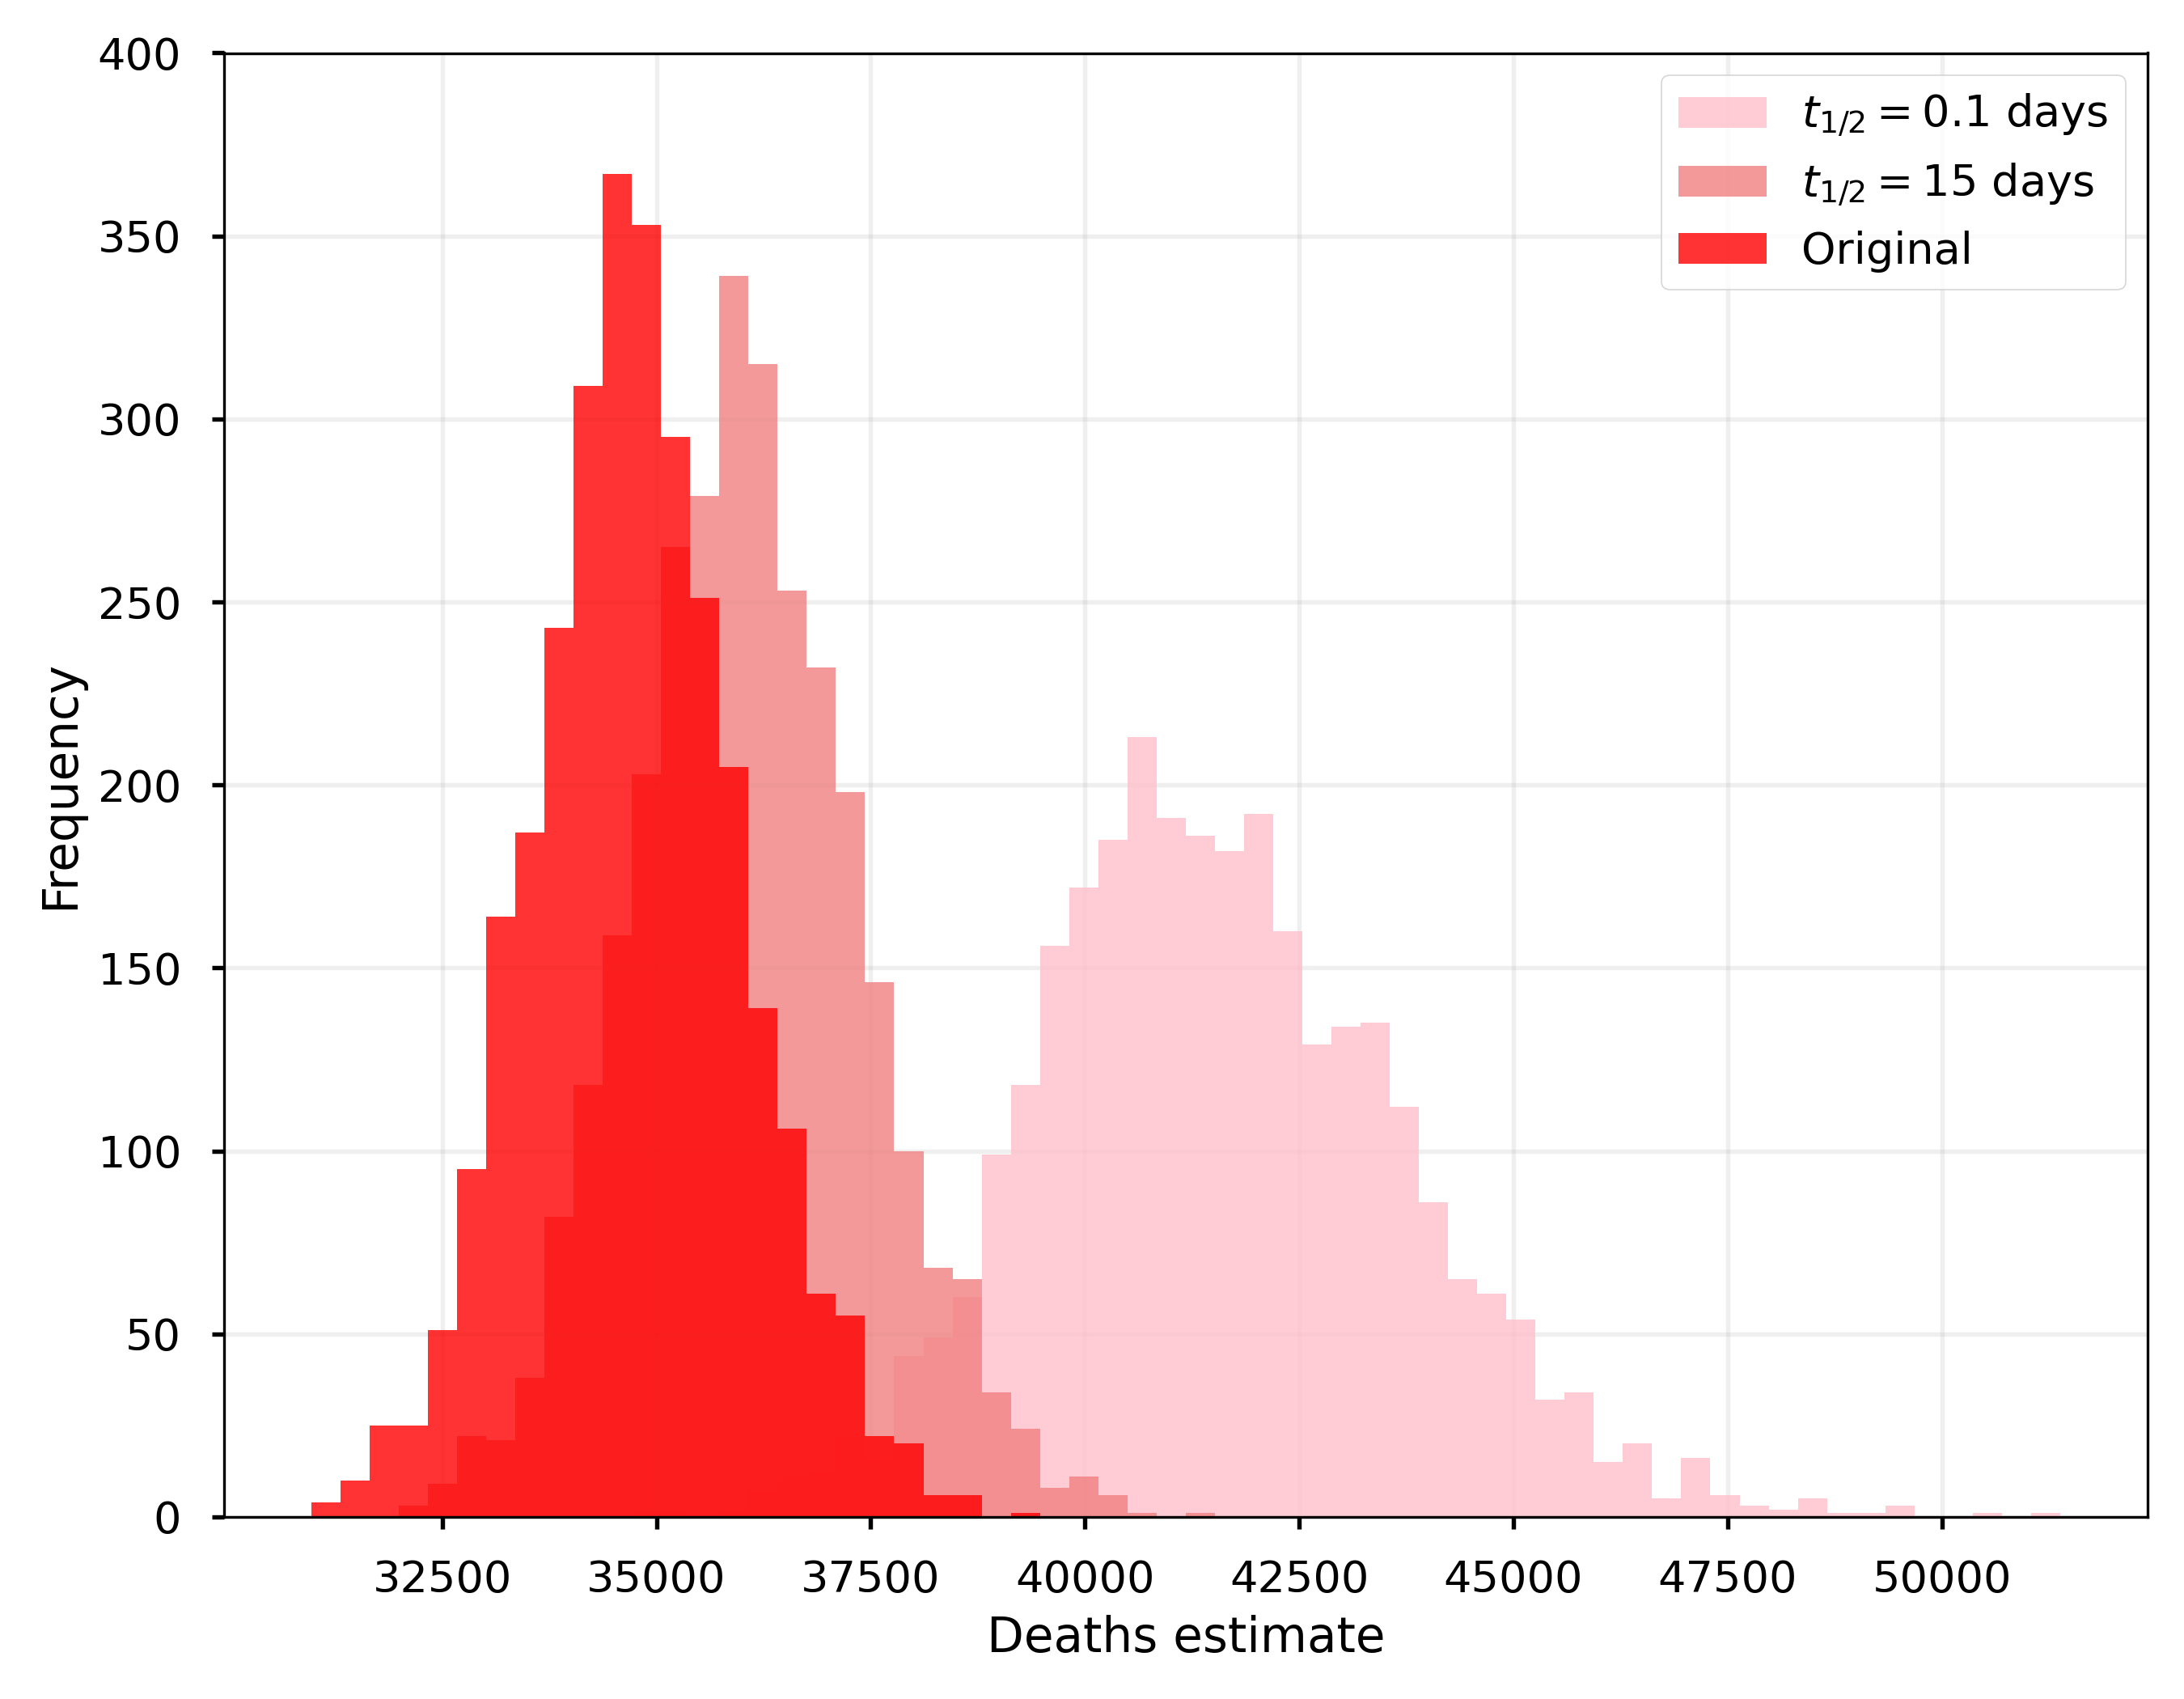
\includegraphics[width=\textwidth]{figs/model_prediction_dead.png}
			\caption*{Death toll}
		\end{subfigure}
	\end{figure}

\end{frame}

\begin{frame}
\frametitle{Results} 
\framesubtitle{Assessing quarantine scenarios} 

	\begin{figure}
		\centering
		\caption*{Effective Reproduction number: relaxation implies in a longer time to disease eradication}
		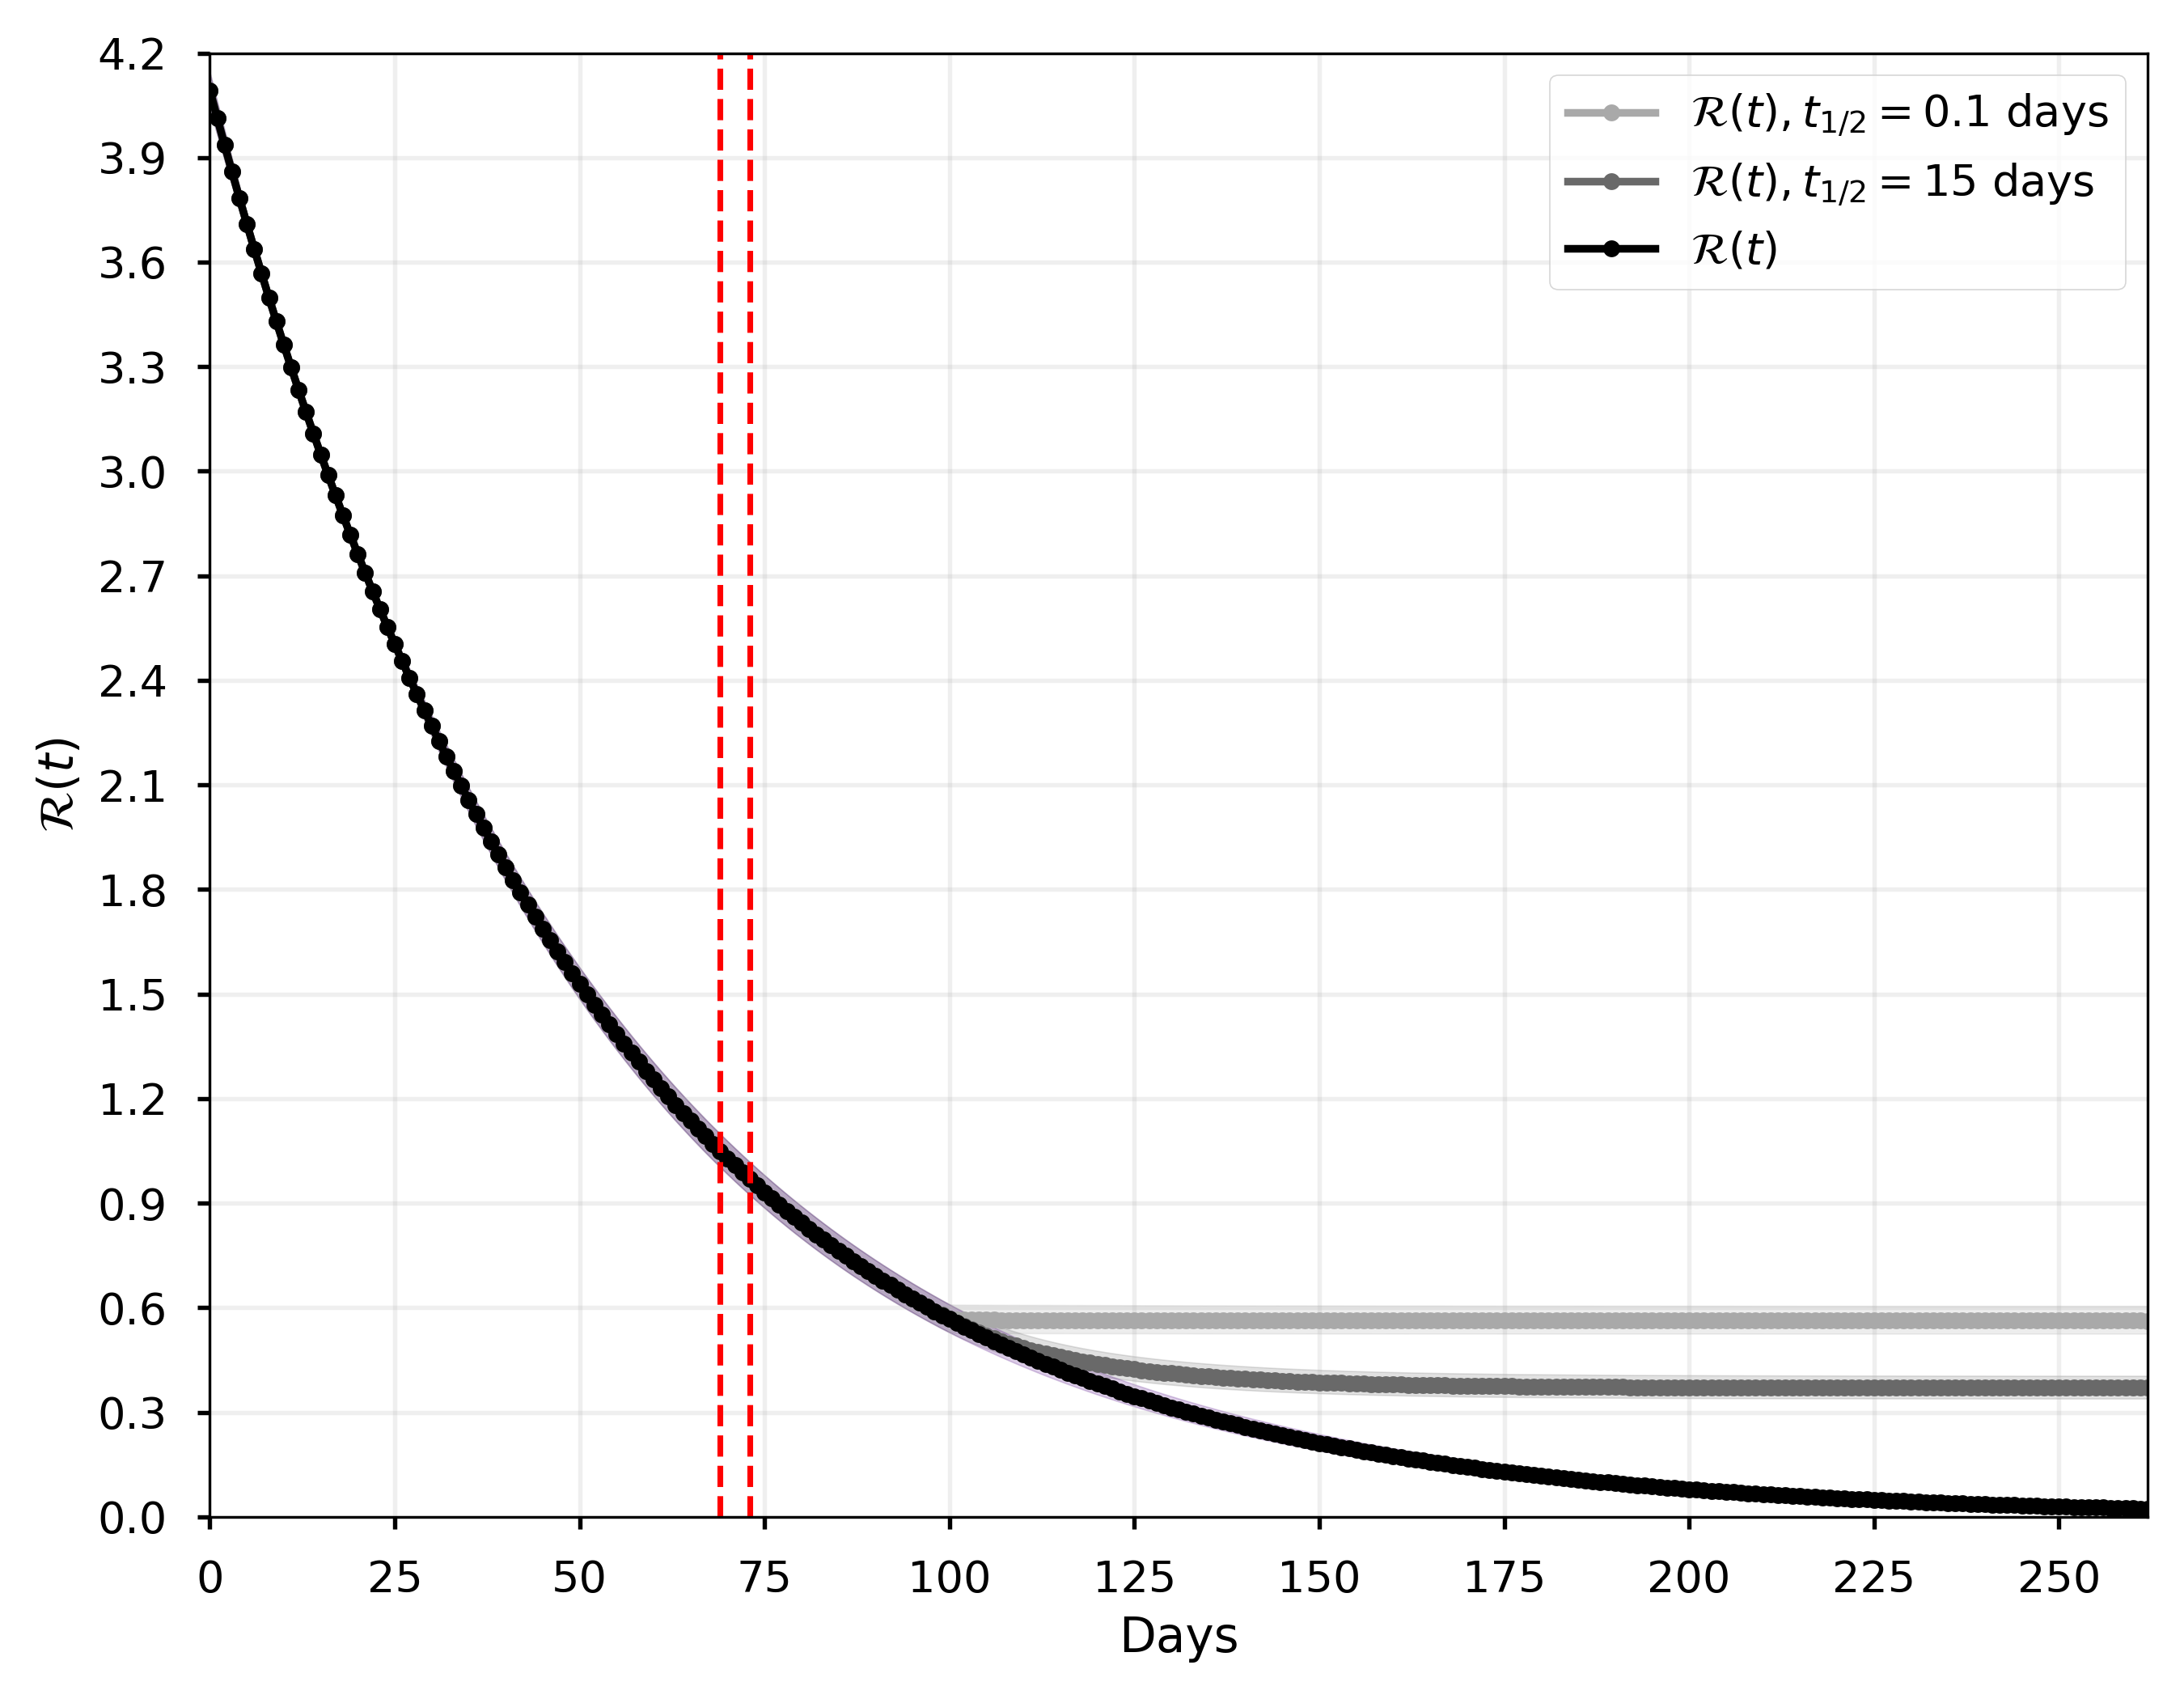
\includegraphics[scale=0.31]{figs/Rt_prediction_bayes_all.png}
	\end{figure}

\end{frame}

\begin{frame}
\frametitle{Results} 
\framesubtitle{Assessing quarantine scenarios}

\only<1-2>{
\begin{center}
    What if quarantine policy relaxation is applied without disease control evidence?
\end{center}
}
    \only<2>{
	\begin{figure}
		\centering
		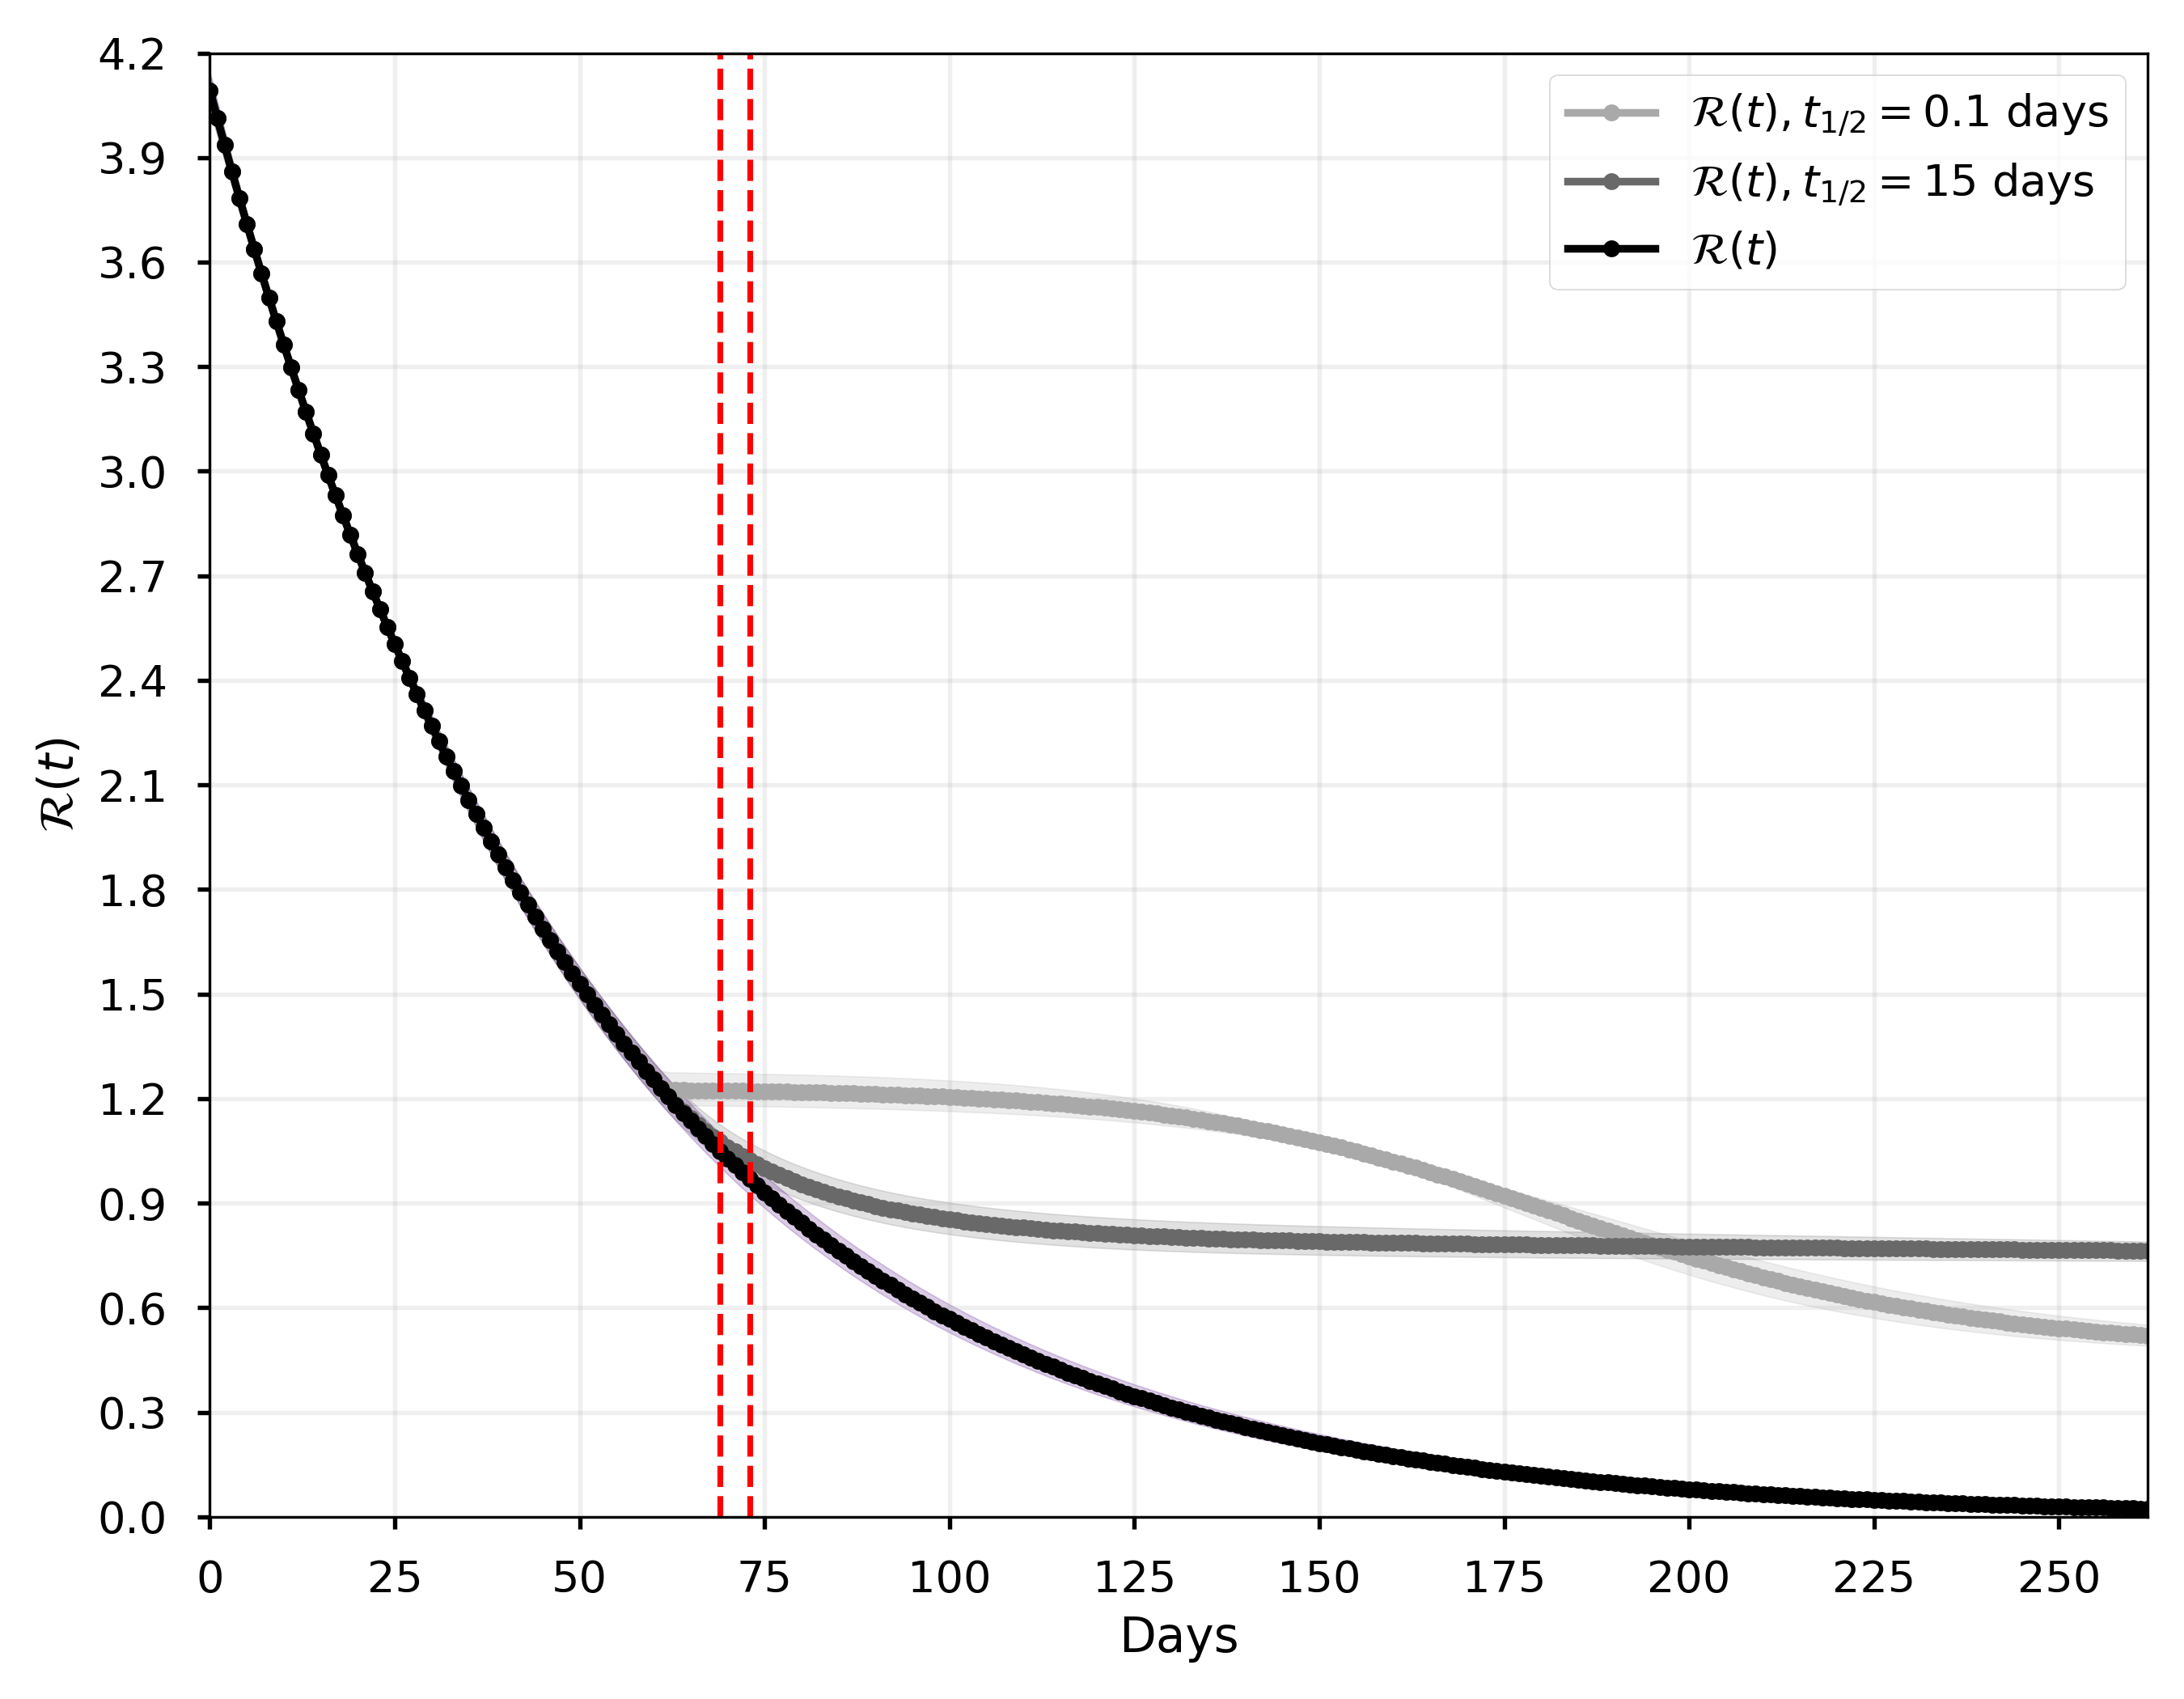
\includegraphics[scale=0.31]{figs/Rt_prediction_bayes_all2.png}
		\caption*{Higher $\mathcal{R}(t)$ for an even longer period, requiring more time to reach $\mathcal{R}(t) \le 1$}
	\end{figure}
	}
\end{frame}

\begin{frame}
\frametitle{Results} 
\framesubtitle{Assessing quarantine scenarios}
	\begin{figure}
		\centering
		\caption*{A terrible scenario is achieved regardless of quarantine policy relaxation strategy}
		\begin{subfigure}[t]{0.49\textwidth}
			\centering
			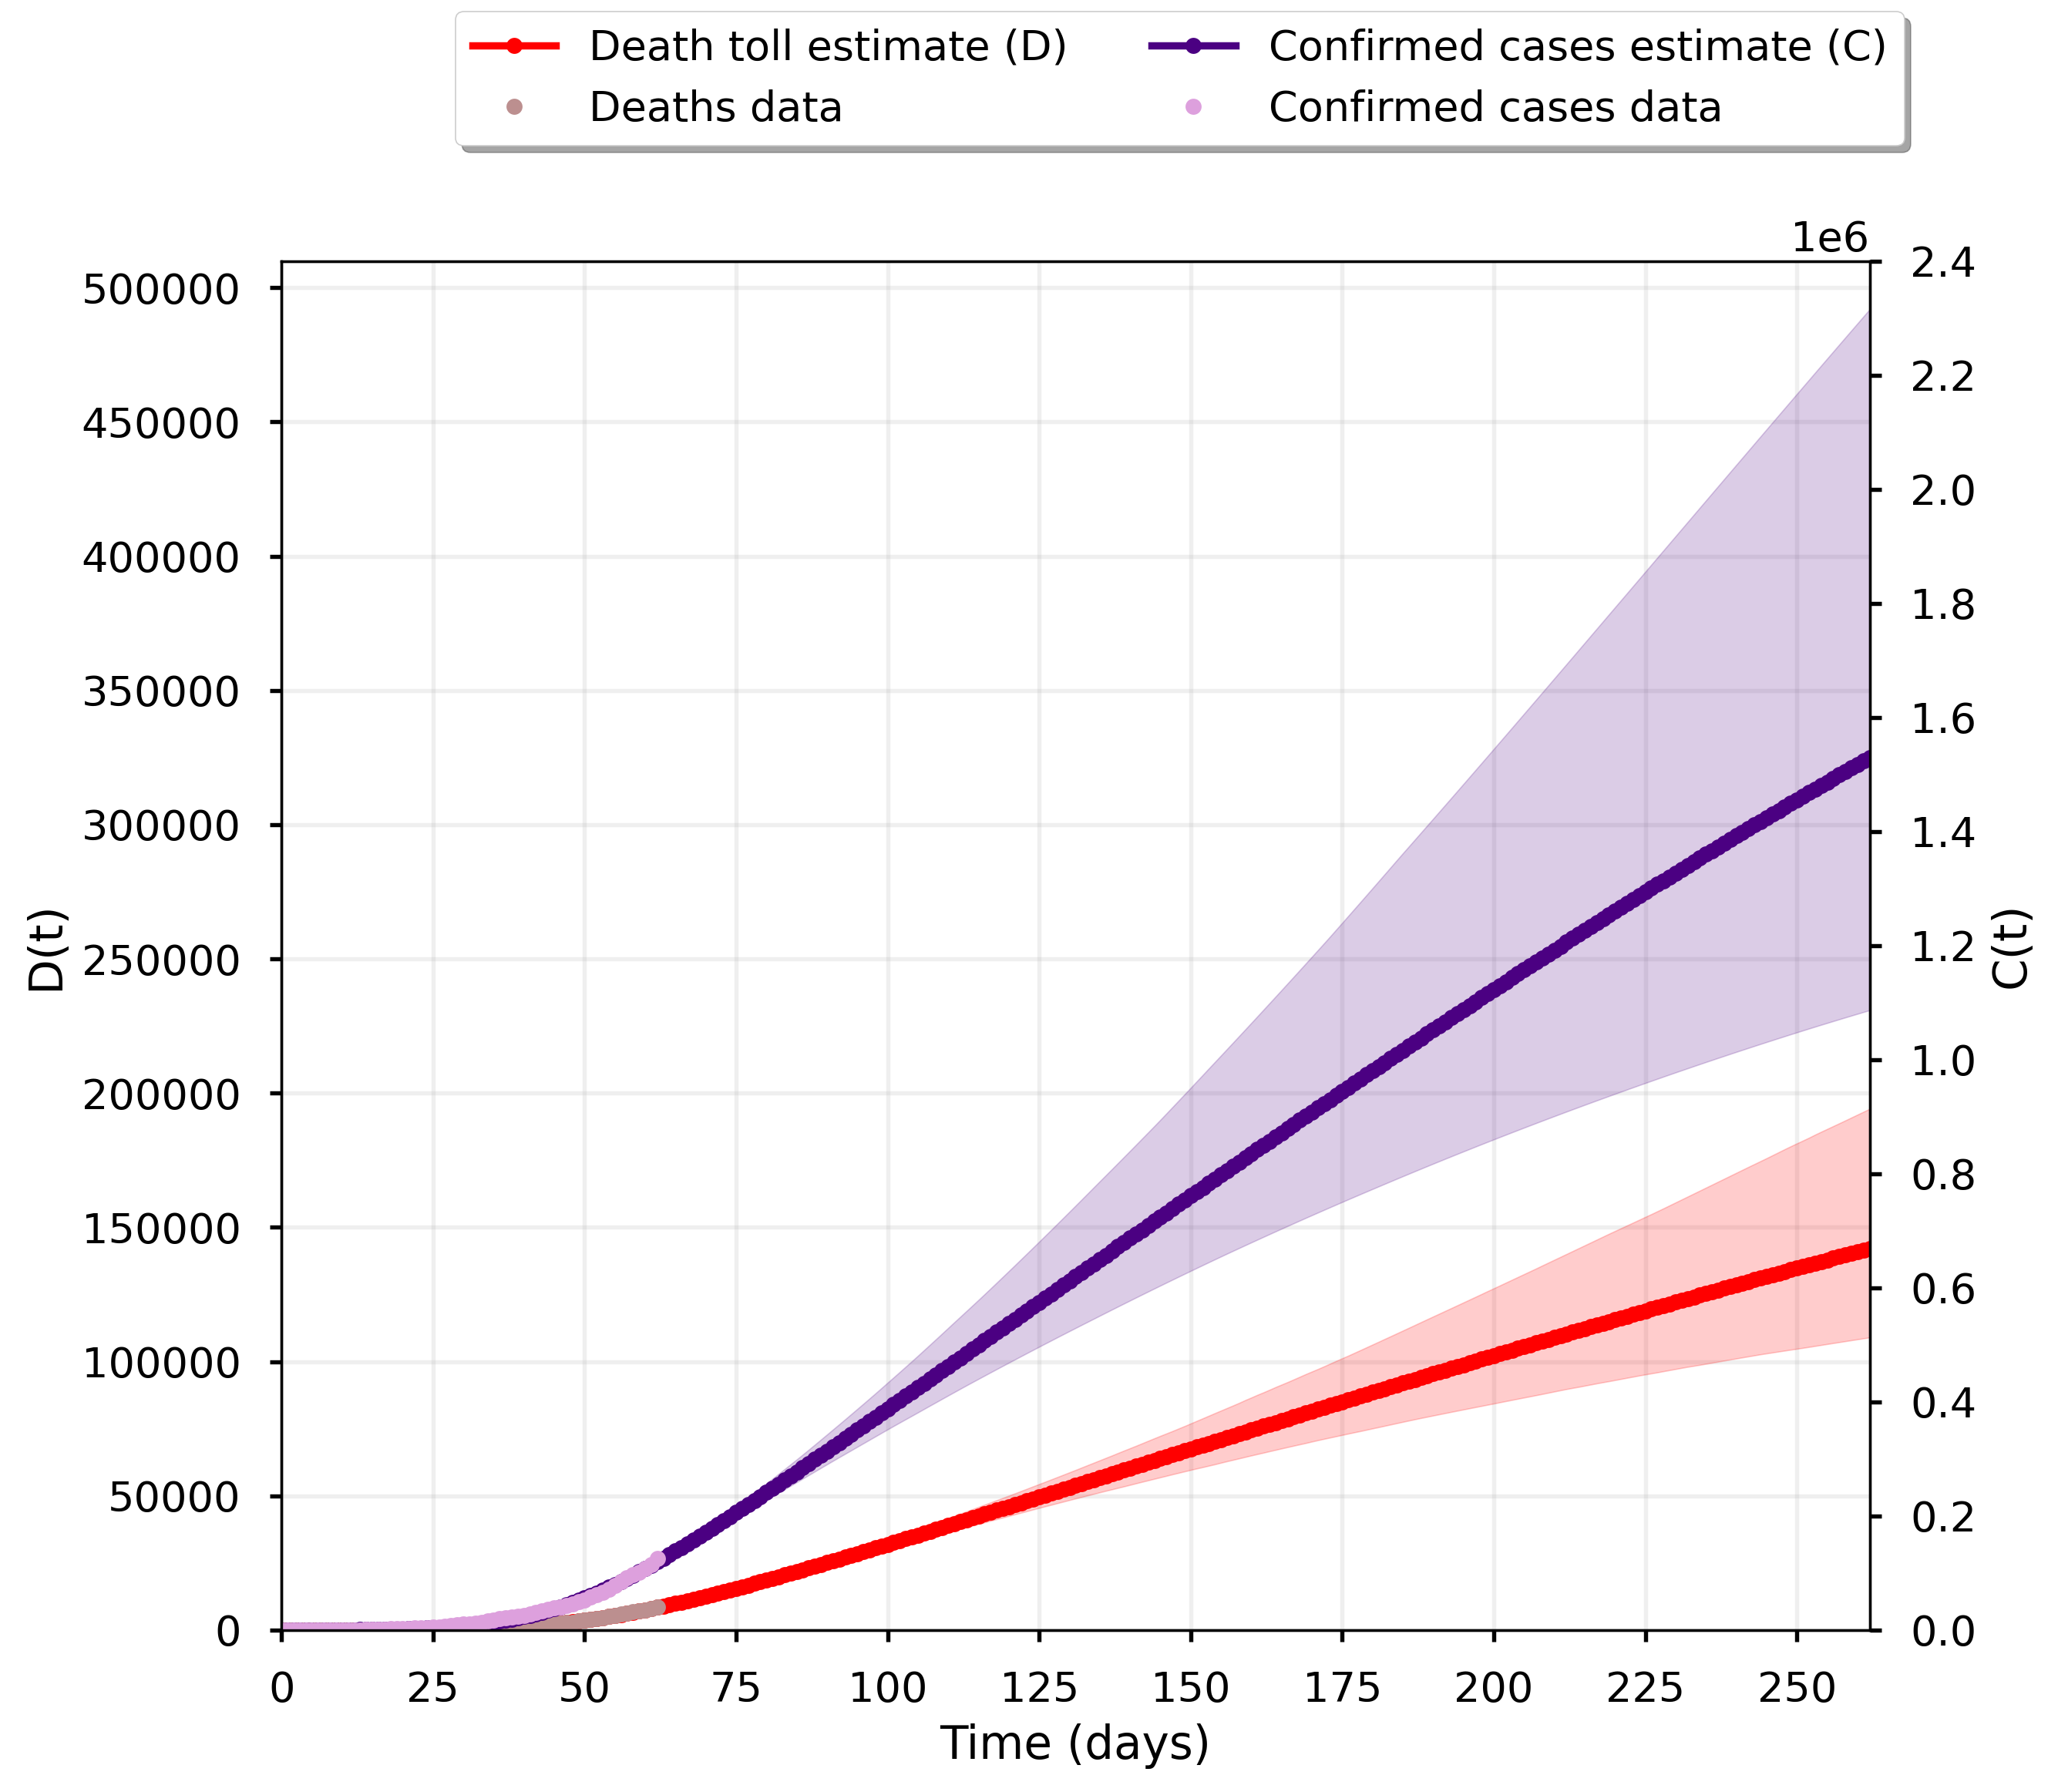
\includegraphics[width=\textwidth]{figs/model_prediction_bayes3.png}
			\caption*{Progressive relaxation}
		\end{subfigure}
		\hfill
		\begin{subfigure}[t]{0.49\textwidth}
			\centering
			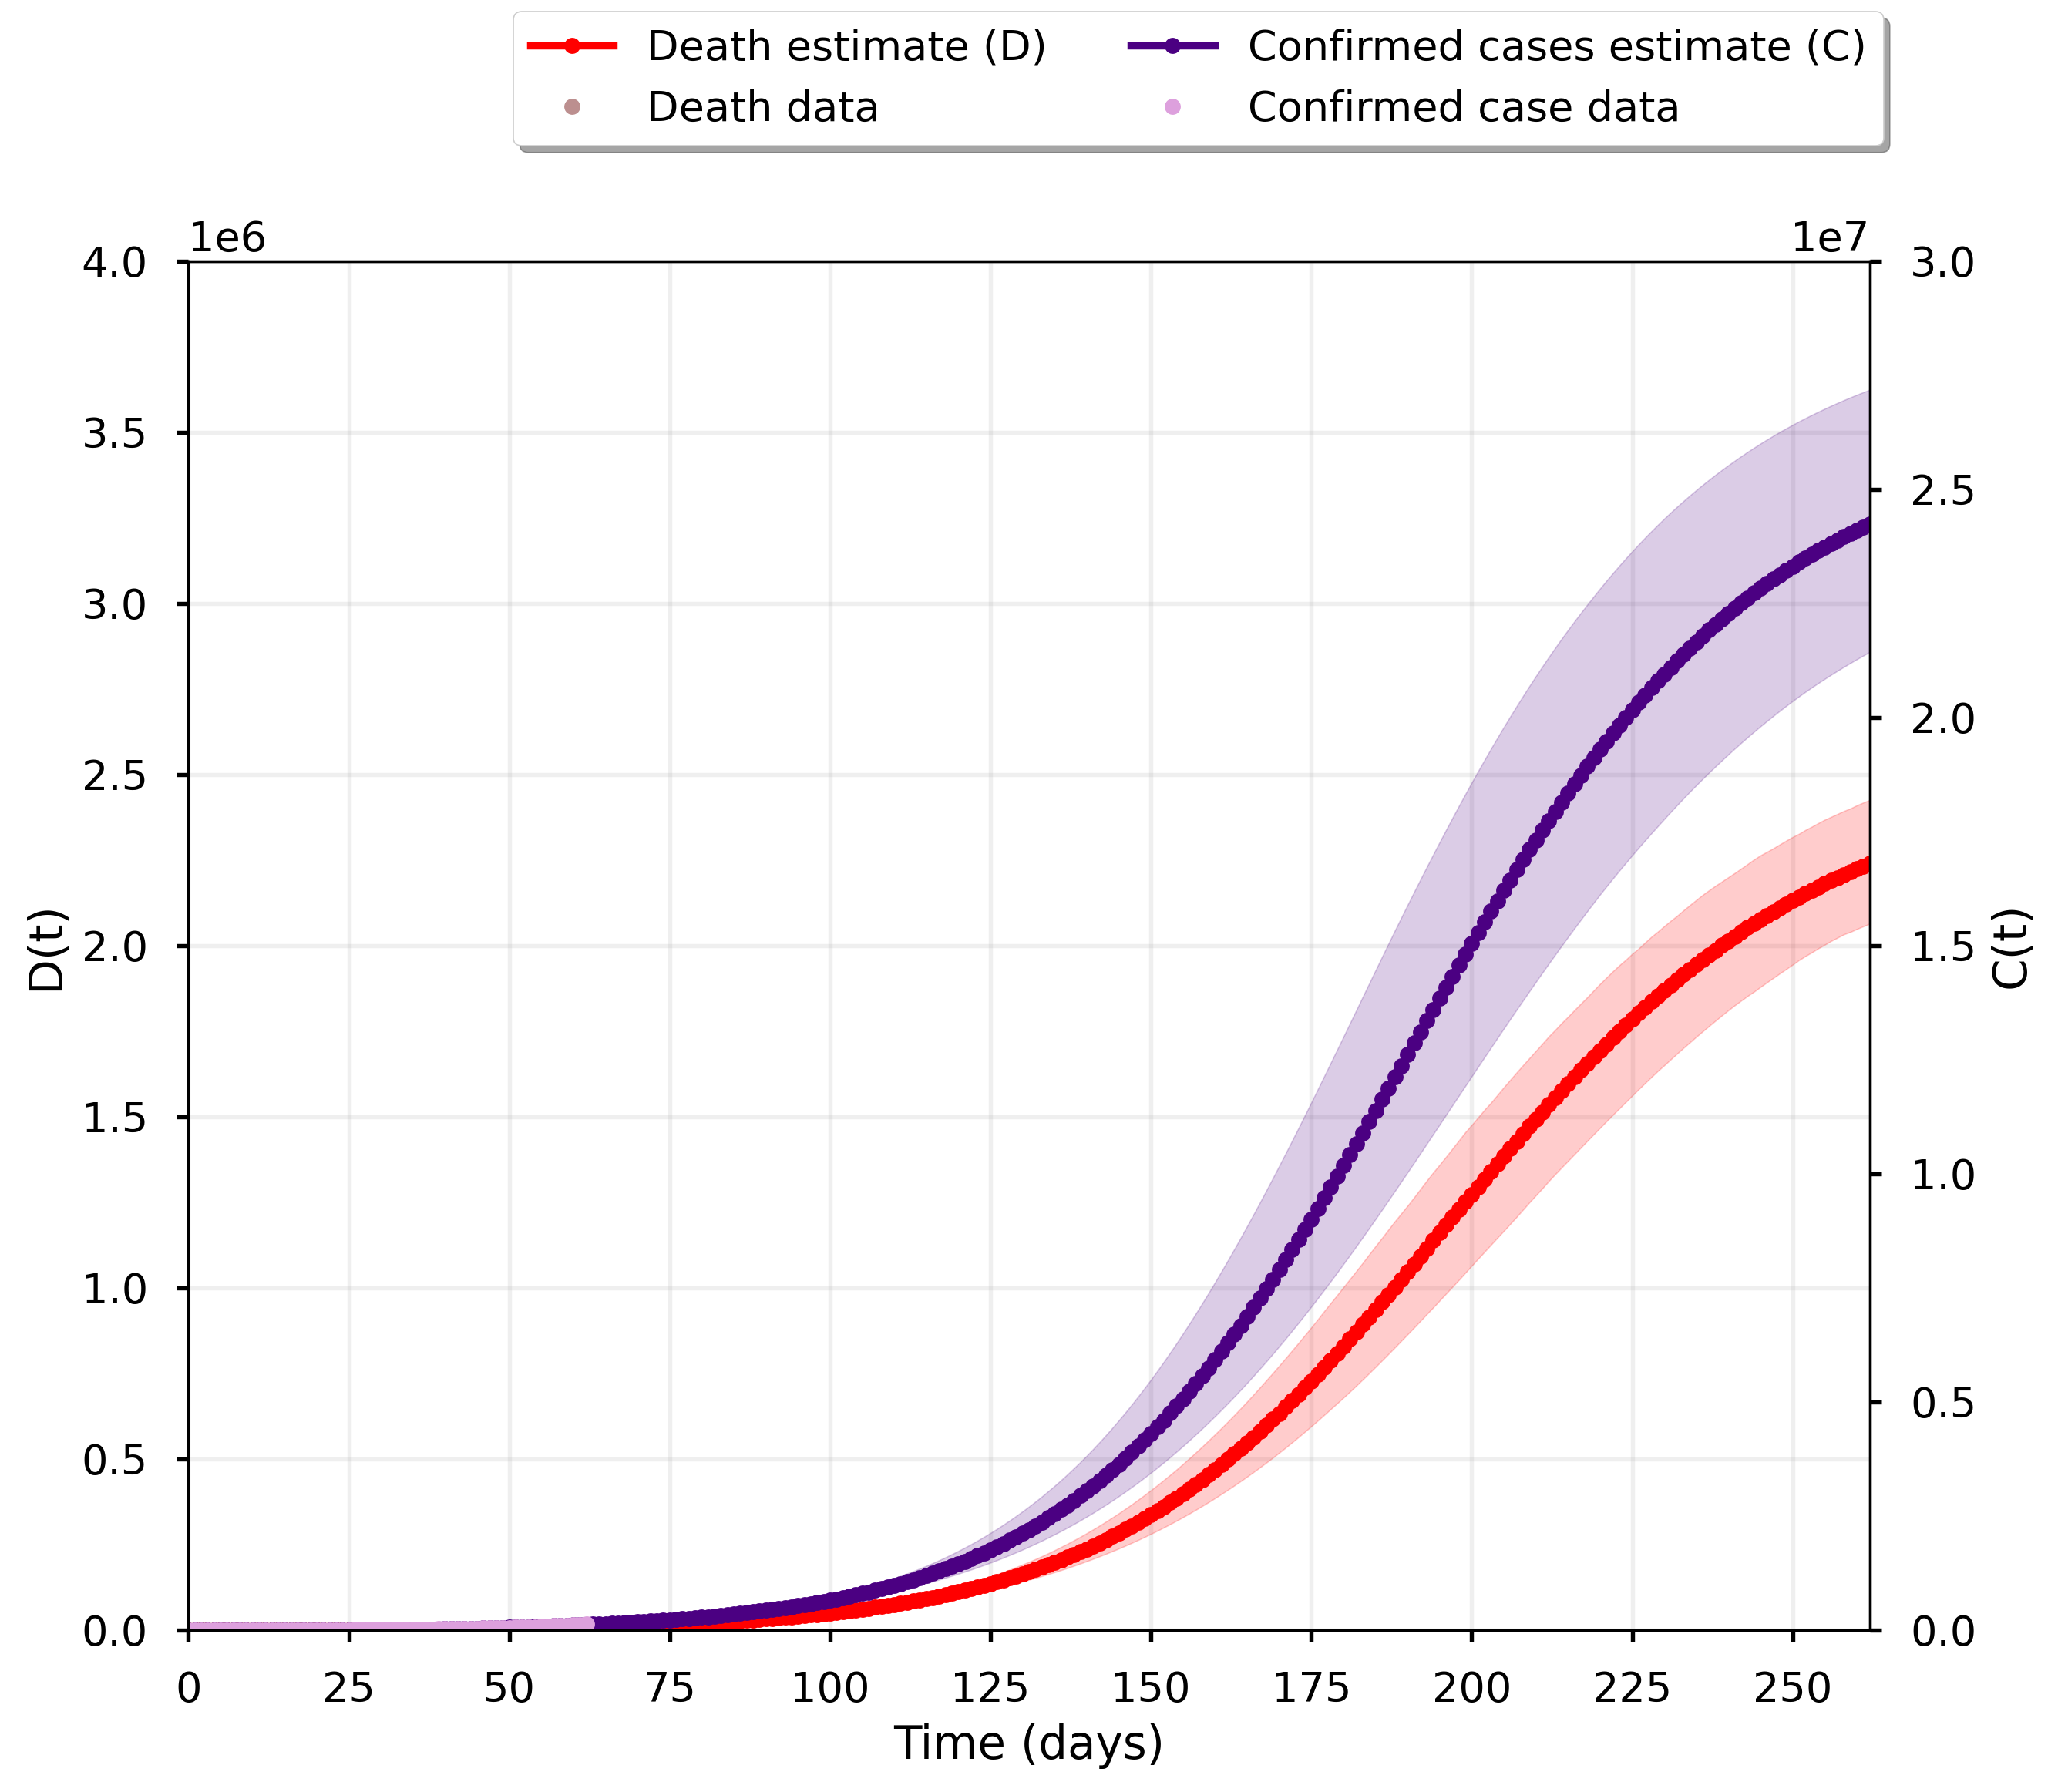
\includegraphics[width=\textwidth]{figs/model_prediction_bayes4.png}
			\caption*{Abrupt relaxation}
		\end{subfigure}
	\end{figure}

\end{frame}

\section{Concluding Remarks}

% \subsection{Our message}

\begin{frame}
\frametitle{Concluding Remarks}
\begin{block}{Main results (and recommendations)}
	\begin{itemize}
		\item Sensitivity analysis suggests that NPIs parameters ($\beta + \mu$ and $\omega$) are the most influential in the disease dynamics
		\item Results show that the maintenance of quarantine policy can help to control the spreading
		\item "Decision timing" plays a fundamental role, even when the "almost under control"
		\item Uncertainties increase in worse scenarios, making the disease control diagnosis more difficult to detect
	\end{itemize}
\end{block}

\end{frame}

\begin{frame}
\begin{center}
    \textcolor{lncc-color}{\Large\textbf{Thank you and stay safe!}}
\end{center}
\vspace{2.em}
\begin{center}
Check out our preprint: "Spreading of COVID-19 in Brazil: Impacts and uncertainties in social distancing strategies" \\
\vspace{1.em}

\includegraphics[height=2.5cm,keepaspectratio]{figs/art.png} \\
\vspace{3em}
\texttt{volpatto@lncc.br}
\end{center}

\end{frame} 

\end{document}